\documentclass[force,almostfull,justified]{tufte-book}
% ------------------history of CASA for Dummies:
%  V1.0  Nadeem
%  V1.1  edited by MBietenholz
%  V1.2  replaced the ^M, use ``verbatim'';  not complete!!
%  V1.3  further modified by MBietenholz; repl ``STAGE'' w/ ``STEP''
%  V1.4  further modified by MBietenholz
%      **** handed out at 2012 Oct workshop
%  V1.5  further corrections + justify document class added
%  V1.7  edit and update of spectral line chapter for by S Goedhard
%  V2.0  edited by MFB and others 2013 Aug.
%  V2.1  added stylesheet and references, bug fixing and cleaning up by R van Rooyen (Jan 2014)

\hypersetup{colorlinks}% uncomment this line if you prefer colored hyperlinks (e.g., for onscreen viewing)

% Book metadata
% \title{CASA for Dummies:\\ A KAT-7 Data Reduction Guide}
\title{Introduction to CASA: \\ A KAT-7 Data Reduction Guide}
\author[Nadeem Oozeer]{N. Oozeer, M. Bietenholz \& S. Goedhart}

\usepackage{casadoc}

\begin{document}

% Front matter
\frontmatter

% r.3 full title page
\maketitle

\vfill
\openepigraph{
\ldots You cannot acquire experience by making experiments. You cannot create experience. You must undergo it.}{Albert Camus.}

% r.5 contents
\tableofcontents
%\listoffigures
%\listoftables

% r.7 dedication
%\cleardoublepage
%~\vfill
%\begin{doublespace}
%\noindent\fontsize{18}{22}\selectfont\itshape
%\nohyphenation
%Dedicated to those who dare to stop going Aips 
%\end{doublespace}
%\vfill
%\vfill


% r.9 introduction
%\cleardoublepage

%%
% Start the main matter (normal chapters)
\mainmatter


\chapter{Why do you want to learn CASA?}
\label{ch:introduction}

For quite some decades, radio astronomy data reduction has been performed using AIPS, Miriad and other
packages.  The coming online of new and substantially enhanced radio interferometers like ALMA, LOFAR
and the JVLA has driven the development of a new software package for interferometric data named CASA.
CASA is better suited to the complexity and data-volume from these instruments than previous existing
packages.  CASA was developed by NRAO, and was built on the Aips++ codebase.  It seems to be becoming
the software suite of choice for radio interferometric data.  KAT-7 is a small interferometer array
and this tutorial presents a guide to reducing the Karoo Array Telescope (KAT-7) data using CASA.
% We will not go into comparing the various packages but rather
% just provide a guide to reducing the Karoo Array Telescope (KAT-7) data
% using CASA.

\begin{marginfigure}
 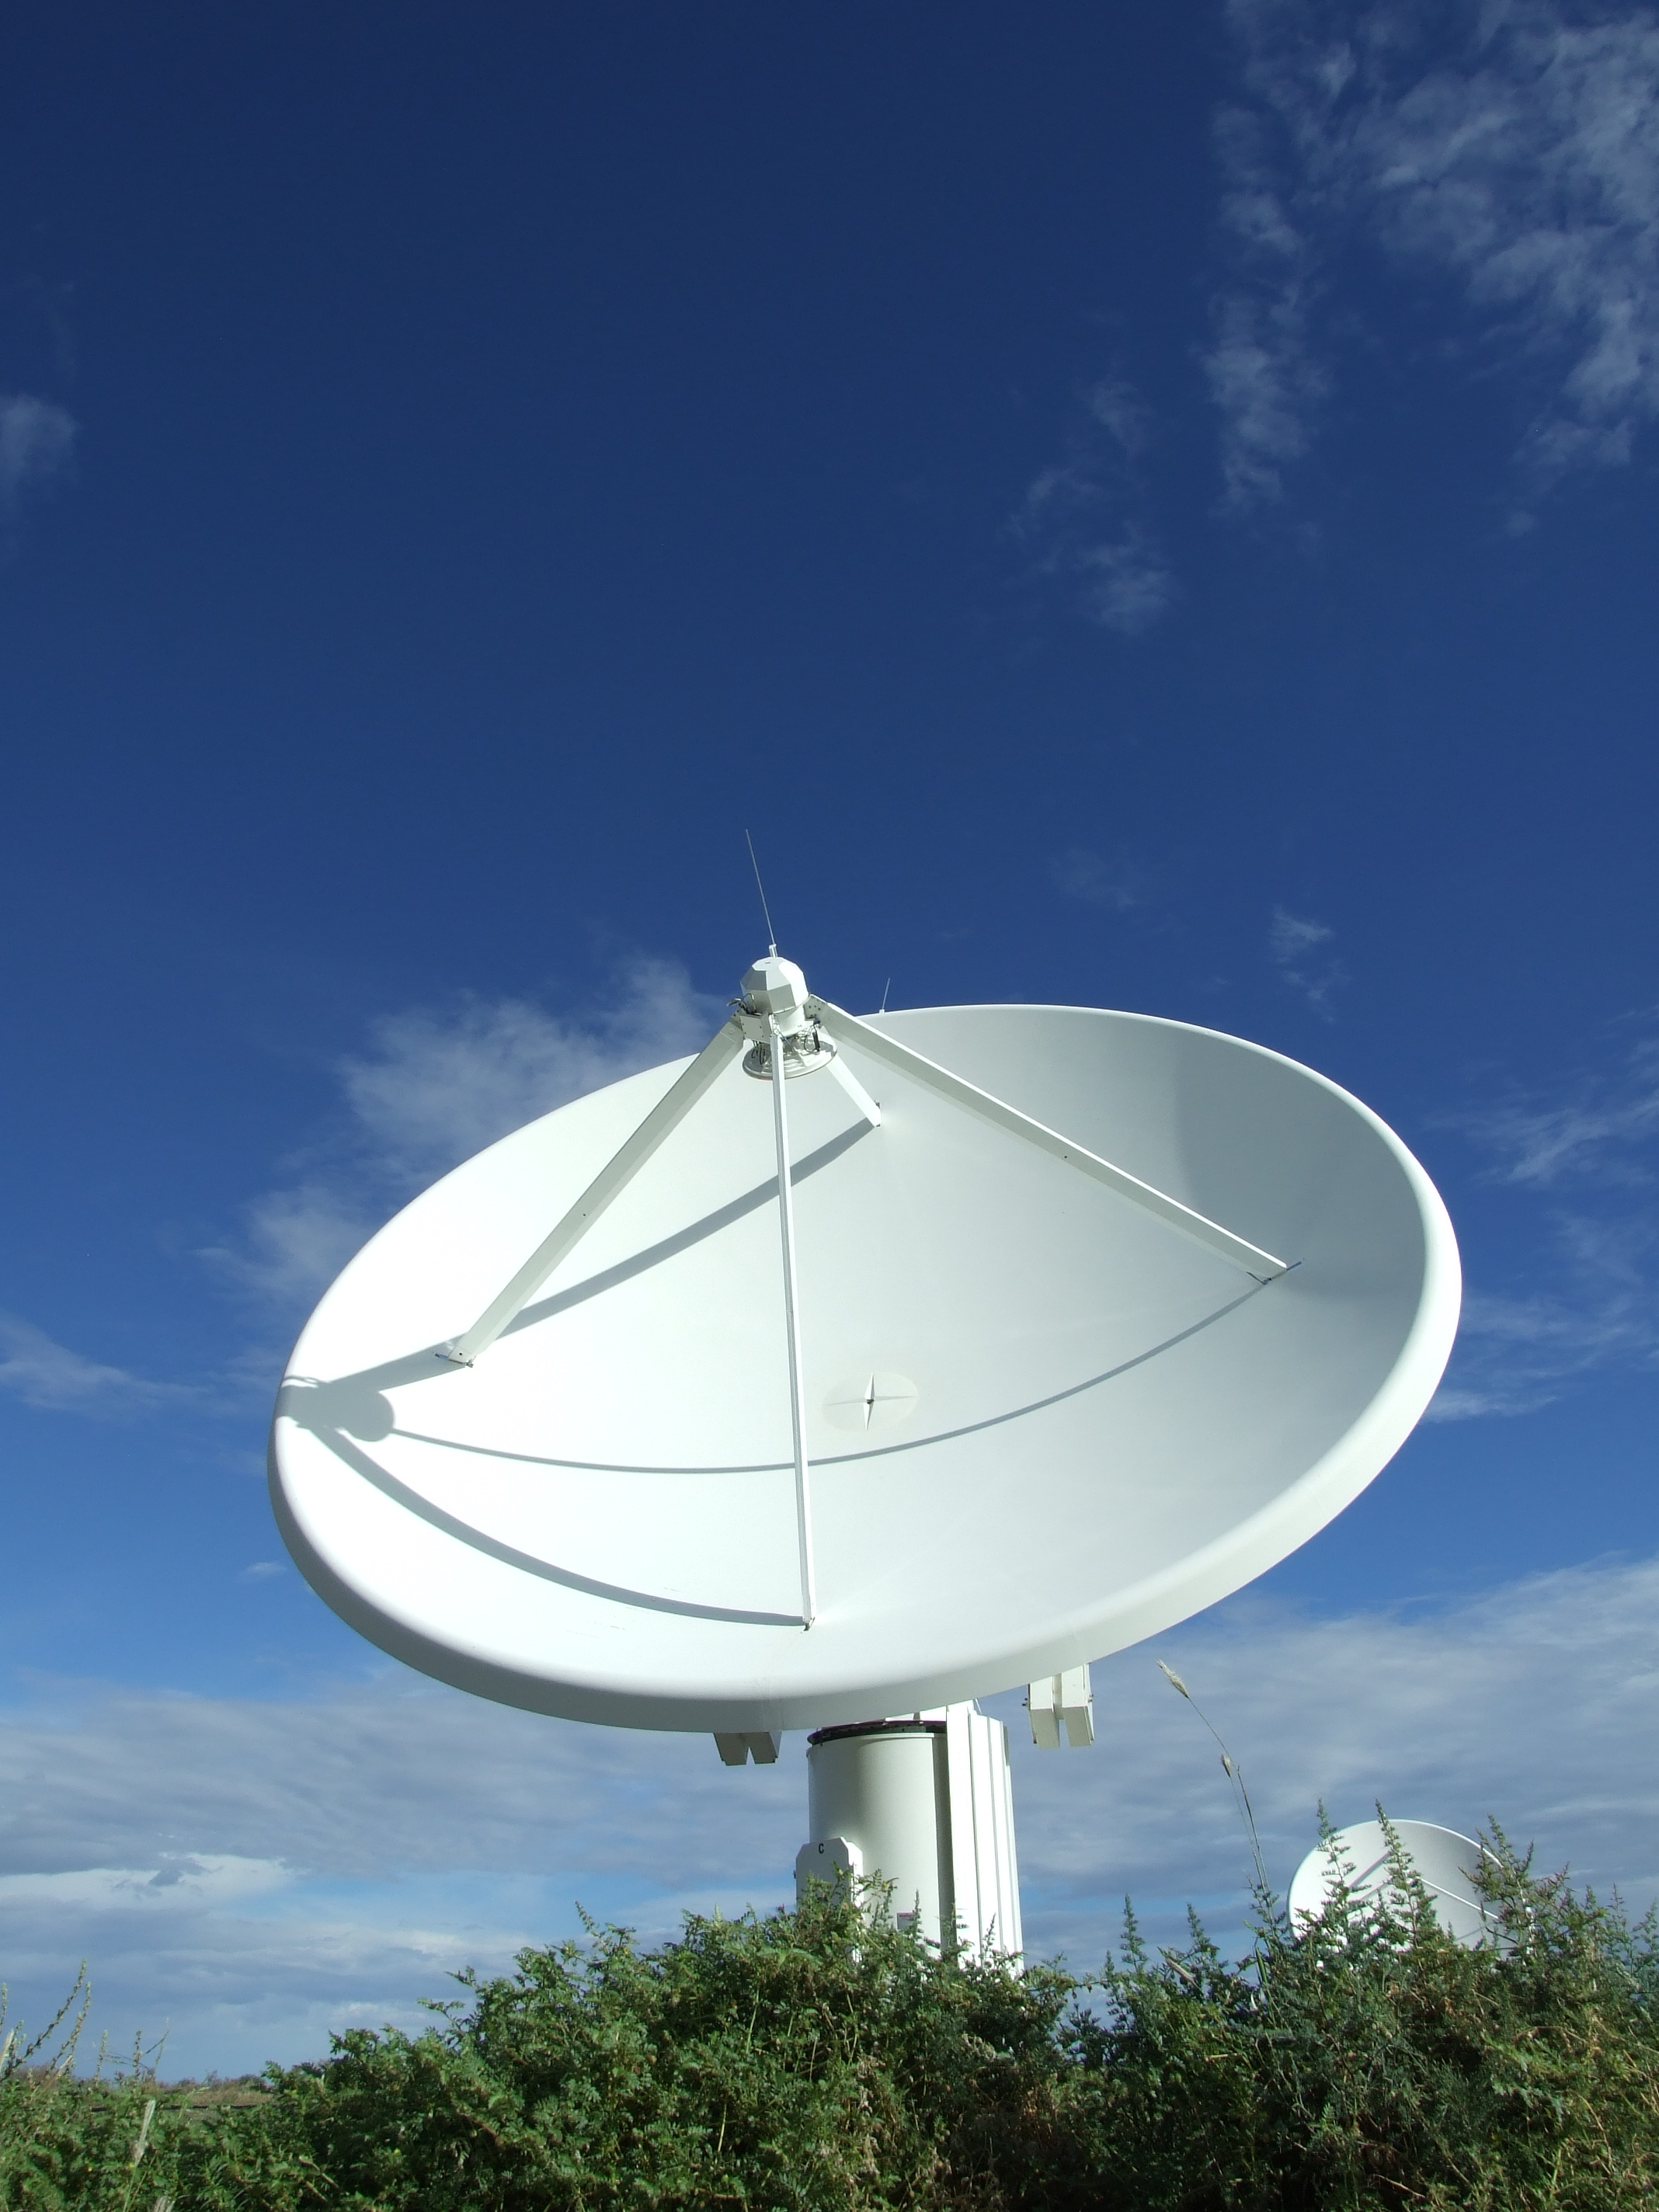
\includegraphics{images/DSCF3329}
 \caption{One of the KAT-7 dishes.}
 \forceversofloat
 \label{fig:marginfig}\end{marginfigure}

Producing an image from interferometer data is not straightforward: an interferometer does not form an
image in the way an optical telescope does, but rather the observations are made in a spatial
frequency space, called the u-v or visibility plane, which is essentially a Fourier transform of the
image plane.  So, in order to make an image, the interferometer measurements must be Fourier
transformed.

Due to the nature of the interferometer, the $(u, v)$ plane is not fully sampled.  The presence of
unsampled regions in the $(u, v)$ causes artifacts to appear in the image plane.  The actual
measurements made by the interferometer are called visibility measurements.  In particular, the
geometry of the telescopes in relation to the direction to the source determines the instantaneous u-v
coverage of an interferometer.  Often the source is observed for some time, and as the earth and the
telescopes on it rotate with respect to the source, the pattern of $(u, v)$ coverage also rotates,
allowing more parts of the $(u, v)$ plane to be sampled. The Fourier transform of this sampling
function is the point-spread function of the instrument, called the ``dirty beam'' in radio
interferometry.

An interferometer is inherently a somewhat complex instrument, and modern radio interferometers all
produce multi-layered data sets which have visibility measurements from all the different baselines
forming the interferometer, possibly of several different polarization products, and in addition, they
often have a large number of independent frequency channels.  Depending in the science aims, these
independent channels can be combined to form a single-channel image, or they can be used to produce a
multi-channel image cube.

However, before the visibility measurements can be sensibly Fourier transformed to the image plane,
they must be calibrated.  Each telescope has a complex gain which is not known a priori, but must be
determined from the observations.  Often specific sources with known properties, called calibrator
sources, are observed with the express purpose of determining these gain factors.  The visibility
measurements on any baseline are affected by the complex gains of both telescopes making up that
baseline.  The first stage of data processing in aperture synthesis is to determine the amplitude gain
and the phase-shift due to each individual telescope (and the atmosphere above it), which together
form the complex gain for that telescope.  Although an interferometer is designed to keep these gains
as stable as possible, they do vary with time, in particular the phase part.

Data sets often also contain some bad or corrupted data, most commonly due to radio frequency
interference (RFI\footnote{\url{http://pos.sissa.it/archive/conferences/107/001/RFI2010_001.pdf}}) or
to malfunction of some part of the antenna electronics.  This bad data should be removed, and the
process of removing them is known as flagging. If the calibration is to be determined from
observations of calibrator sources, then any bad data for the calibrator sources should ideally be
removed before determining the calibration solutions.  For other sources it is generally easier to
identify bad data after the calibration is applied.

Once the visibility data are properly calibrated and edited, they can then be Fourier transformed to
make an image.  However, due to the incomplete sampling in the image plane, the image so produced is
the convolution of the sky brightness with the point spread function of the interferometer, which is
called the ``dirty beam''.  The second part of the data reduction is to try and correct the image, to
the extent possible, for the effects of this incomplete sampling.  Unlike data at some other
wavelengths, radio data can require hours to days of reduction to achieve the highest dynamic range.
Ideally, the image meets the constraints of physical consistency as well as plausibility.  This
document will attempt to explain the various stages for getting radio images from KAT-7 data.


\section{How to use this document}

This document assumes that you are conversant with Linux and Python. If not, then the book ``SAMS
teach yourself Linux in 10 minutes'' will be a good start even though you will take more than 10
minutes to read the whole book.  Reading ``Python for Dummies'' will also help. We will also not cover
all the fundamentals of radio astronomy, but from time to time we shall try to discuss some concepts
before proceeding so that the user is aware of what we are doing.  For a thorough introduction to the
fundamentals of radio astronomy, we recommend the NRAO Essential Radio Astronomy online course
(\url{http://www.cv.nrao.edu/course/astr534/ERA.shtml}).

The procedures consist of various steps and each step generally depends on the previous ones. So avoid
skipping to the next step if you have warnings and errors, without clearing them.  We will note those
steps that are independent of the preceding ones.


\section{Conventions used}
We have tried to use the following conventions through this document:

\begin{itemize}

\item A {\tt typewriter font} is used for CASA tasknames and variables in the main text, and for CASA
input and outputs given in a red box, for example:

\begin{casacmd}
\begin{verbatim}
prefix = 'CirX1'
msfile = prefix+'.ms' 
\end{verbatim}
\end{casacmd}

\item The Return key is synonymous with the ENTER key or $\hookleftarrow$

\end{itemize}

\info{Tips: lead to shortcuts that we find useful}

\caution{Cautions: Avoid pitfalls}

\comment{Comments: explain the relevant procedure}

\pause{Pause: Time for a break}


\section{Methodology}

In this document we will review the data reduction procedures that we will use during the in-house
workshop on CASA.

\begin{figure*}
  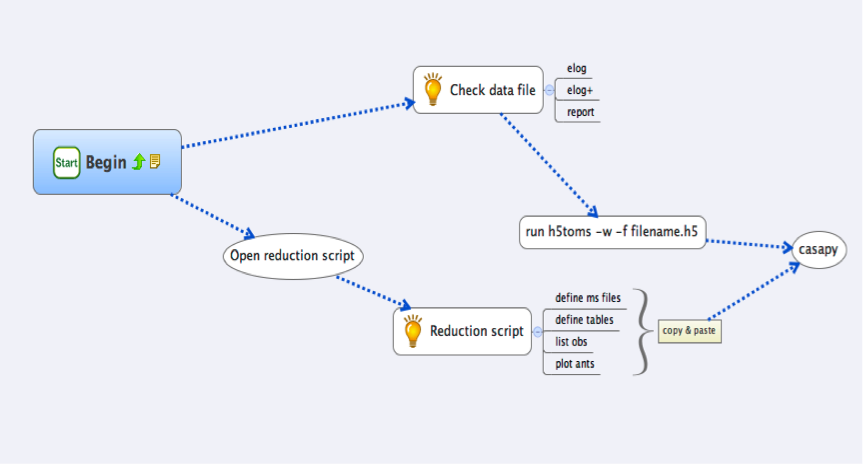
\includegraphics[width=12cm]{images/casa_begin}
%  \checkparity This is an \pageparity\ page.%
  \caption[Mind map.]{This mindmap shows the routes for getting your data into CASA}
  \forceversofloat
  \label{fig:casa_begin}
  %\zsavepos{pos:textfig}
\end{figure*}

Before you begin in this long journey of data reduction, make sure you have enough time to spend. It
can get very crazy; get lot of snacks, coffee and put THE sign (Figure~\ref{fig:marginfig_disturb}) in
a place clearly visible to the rest of the world. Basically we expect for a newbie to spend around 3-5
days to successfully reduce a KAT-7 dataset.  However, this documentation will allow you to get a
clean image in a day, the target is within 10 hours of CONTINUOUS work.

It is not that hard but requires lot of attention and concentration. The process will become quicker
after you've worked with a few data sets and have become familiar with it.

OK let us get serious now.

\caution{
   Python is case sensitive (as is Linux).  Always ensure 
   you using the correct case.
}
  \begin{marginfigure}[-5.0cm]
  \begin{center}
 
\includegraphics[width=7.5cm,height=9.5cm]{images/Do_not_disturb} 
 \caption{THE sign}
 \forceversofloat
 \label{fig:marginfig_disturb}
 \end{center}\end{marginfigure}

%% - RVR -- Remove chapter = Section 1.1 refers to python references
% \chapter{Python a crash tour}
% \label{ch:python}
% \TODO


\chapter{Let us get serious}
\label{ch:let_get_serious}


\bigskip
\section{Overview of Calibration}
% the \emph *turns off* the italic here

The visibility measurement made by the interferometer are complex values, having either real and
imaginary parts, or an amplitude and a phase.  The calibration process consists mostly of finding a
set of time and frequency dependent complex gain factors, by which our visibilities need to be
multiplied.

We develop our complex gain solution in stages.  Some parts vary with time but not so much with
frequency, for example transmission through the atmosphere causes both phase shifts and attenuation.
However, the variation of the atmospheric part of the complex gain across the observing band is
usually small.  Therefore, a combined solution for all the different frequency channels of
observations is usually possible.  The bandpass response of the instrument, by contrast, varies across
the frequency band, but is usually quite stable in time, so that it needs to be solved for only once
in an observing run.

So our whole set of complex gain factors is usually broken up into several pieces, each of which is
solved for separately.  This division is not necessarily unique, in the end all that matters is the
complex product of the individual parts of the calibration.

% MFB removed this 2013 Aug 21 - I think its leftover from somewhere
%The typical bits are usually these:
%
%\begin{itemize}
%\item{Delay calibration} Large changes in the propagation delay
%of the signals to different antennas.  For KAT-7 data this usually
%only needs to be solved for once, as the delays are expected to be
%\end{itemize}

\bigskip
\section{STEP 1... Converting the hdf5 file to a MS}

Note that for the data set we are using for the tutorial, this step has already been done, so you can
skip ahead to the next section.  If you need to do this step, go to the KAT-7 archive to search for
your file.  Then check the eLog to see if the telescope operator entered any information during the
observations, and take note of any if they did.  Then, proceed to converting the archive file to a
Measurement Set (ms).  An ms is the form in which CASA will work on your data.  Also remember at the
end of the data reduction to add an entry in the eLog of the results.  Convert the hdf5 archive file
to an ms using the in-house script {\tt h5toms} as follows:

\bigskip
\linuxcmd{h5toms.py -f --no-auto -C '199,799' --flags='all' -r ant5 myfile.h5}

The {\tt -f} flag causes {\tt h5toms.py} to produce a full-polarization output file, while the {\tt
no-auto} causes {\tt h5toms} to load only cross-correlations, but not the auto-correlations.  The {\tt
-C 199,799} flag causes {\tt h5toms} to load only channels 199 to 799 (inclusive) of the original 1024
channels. The $\sim$200 channels at either edge of the band are known to be bad, so we do not load
them.  We have also applied the online flagging using the {\tt -{-}flags='all'}.  The {\tt -r ant5}
causes it to use antenna 5 as the reference antenna (although you can change this later if required).

The output will be a directory {\tt myfile.full\_pol.ms}. This directory is your CASA measurement set.
More options are available for {\tt h5toms.py}\footnote{{\tt h5toms.py -h} lists the additional
options e.g.  for {\tt h5toms}}.  Once the data has been successfully converted into an ms, one can
start CASA from the computer kat-imager2 (assuming you are running on the SKA Pinelands server), and
then proceed with the data reduction.

It's probably a good idea to rename your ms to something a little more descriptive at this stage.

\bigskip
\linuxcmd{mv myfile.full\_pol.ms School\_data\_av.ms}.

Of course if you're looking at real data its probably a good idea to use a name for the ms which
reflects what the observations are.

\bigskip
\section{STEP 2... Loading and inspecting the data}

It is probably best to create a specific directory which will contain the working CASA data.  We will
use the directory ``my\_working\_directory''.

%% Added by Ruby, seems to be a missing step of creating the directory
\linuxcmd{mkdir my\_working\_directory}

\smallskip
The first main step is to move the ms into your chosen working directory, and then also to make the
working directory your current directory.  For the workshop, you may have downloaded the file \\ {\tt
School\_data\_av.ms.tar.gz}, which you would unpack with the linux command:

\smallskip
\linuxcmd{tar -zxf School\_data\_av.ms.tar.gz}

\medskip
It should produce a directory called {\tt School\_data\_av.ms}.  This directory is your CASA
measurement set.

\smallskip
\bigskip
\comment{
    Locate the ms directory from the previous step and move it
    into the working directory. 

    \texttt{mv myfile.full\_pol.ms my\_working\_directory} \\
    \texttt{cd my\_working\_directory}
}

\bigskip
\comment{
Although CASA measurements sets (ms) are ordinary linux directories, and can be renamed, moved,
delected or copied like any other directories, there are probably restrictions you should observe:
\begin{itemize}

\item Do not move, delete etc.\ directories from the operating system
  {\em while casapy is running}, as casapy does some ms caching, and
  will likely get confused. You can remove an ms from within casapy by
  typeing e.g., \texttt{rmtables('crappy-data.ms')} and it will be fine,
  or you can just exit casapy and then delete it.

\item Do not alter the {\em contents} of the ms.  While renaming or
  moving the ms directory is fine, its probably not a good idea to add
  or delete any files to the ms, or to alter or rename any of the
  files contined within it.
\end{itemize}
}

\bigskip
\bigskip
Most of the data reduction will be done from within casapy, which provides an interactive shell
(essentially the equivalent of interactive python or ipython). From the Linux prompt you will
therefore first run casapy.  You will then give the commands to run various CASA programs from within
casapy.  In casapy you can also create variables, assign values to them, and then subsequently use
them at any time during the processing.  It is generally convenient to define some variables to hold
the names of ms's and tables.  The sequence of casapy commands can then be re-used for a different
data set by merely changing the values assigned to these variables.

\bigskip
\caution{
   Do NOT abort running programs by pressing Ctrl+C as CASA has a bug and
   will screw up all your visibilities. Rather wait for the command to be
   over and then undo the wrong steps.
}

\bigskip
In fact, CASA is designed to be highly script-able, and sequences of commands could be placed in a
script and run automatically.  In this session, however, we shall be using step-by-step commands.

\bigskip
\caution{
   Never delete the ms file unless you have finished splitting your
   relevant data and are sure you do not need the ms anymore.
}

\bigskip
Below we define a variable to hold the ms (directory) name but without the ``ms'' extension.  We will
use this variable to refer to the ms and to various associated tables.  The ms we are using in the
tutorial is called {\tt Cirx1\_school.ms}, so we define the following variables in casapy:

\bigskip
\begin{casacmd}
\begin{verbatim}
prefix = 'Cirx1_school'
msfile = prefix+'.ms'
\end{verbatim}
\end{casacmd}

\bigskip
We now define variables that hold the names of various tables that will be used during the reduction.
The table names could be specified directly, but if you do it by means of variables, the subsequent
commands we use can be copied and pasted and re-used for some other reduction with the only
modification required being the re-definition of these variables.

\begin{casacmd}
\begin{verbatim}
bandpass_table0 = prefix +'_spw0.B0'
gain_table0 = prefix+'_spw0.G0'
gain_table1 = prefix+'_spw0.G1'
flux_table1 = prefix+'_spw0.fluxscale1'
\end{verbatim}
\end{casacmd}
% %MFB removed defn. of bandpass_table10 as it is never used

We chose antenna {\tt ant5} as our reference antenna when we first converted the data-set to an ms,
because it seems to have more shielding for RFI from the pedestal.  Since it is best to use a
consistent reference antenna throughout, we again define a variable whose value is the current
reference antenna.

\begin{casacmd}
\begin{verbatim}
reference_antenna= 'ant5'
\end{verbatim}
\end{casacmd}

Next, we use the task {\tt listobs} to print out a summary of the observations in the ms (similar to
the AIPS task LISTR with OPTY='SCAN'):

\begin{casacmd}
\begin{verbatim}
listobs(vis=msfile)
\end{verbatim}
\end{casacmd}

% okay new data set
%  all ants have data for two calibratro srcs
%\begin{fullwidth}

\begin{casaoutput}
(we have removed the leading part of the lines of the {\tt listobs} output
for clarity.)
\begin{verbatim}
================================================================================
           MeasurementSet Name:  /home/michael/casa-workshop2012/CirX1.ms      MS Version 2
================================================================================
   Observer: lindsay     Project: 20120701-0006  
Observation: KAT-7
Data records: 71904       Total integration time = 56296.5 seconds
   Observed from   01-Jul-2012/13:57:43.4   to   02-Jul-2012/05:35:59.9 (UTC)

   ObservationID = 0         ArrayID = 0
  Date        Timerange (UTC)          Scan  FldId FieldName           nRows   Int(s)   SpwIds 
  01-Jul-2012/13:57:43.4 - 13:59:27.9     1      0 PKS 1934-638        168    14.1     [0]                         
              14:00:13.4 - 14:04:58.4     2      1 Circinus X-1        420    14.8     [0]                         
              14:05:28.4 - 14:06:21.4     3      2 PKS 1613-586        105    11.6     [0]                         
              14:06:44.5 - 14:11:30.5     4      1 Circinus X-1        420    14.8     [0]                         
              14:12:00.5 - 14:12:45.5     5      2 PKS 1613-586        84     14.5     [0]                         
\end{verbatim}
\dots (we omit the bulk of the detailed scan listing here)
\begin{verbatim}
              05:29:53.8 - 05:30:38.9   328      2 PKS 1613-586        84     15       [0]                         
              05:30:56.9 - 05:31:41.4   329      2 PKS 1613-586        84     14.5     [0]                         
              05:31:58.9 - 05:32:43.9   330      2 PKS 1613-586        84     15       [0]                         
              05:33:01.9 - 05:33:46.9   331      2 PKS 1613-586        84     14.8     [0]                         
              05:34:04.9 - 05:34:49.4   332      2 PKS 1613-586        84     14.8     [0]                         
              05:35:06.9 - 05:35:59.9   333      2 PKS 1613-586        105    12       [0]                         
           (nRows = Total number of rows per scan) 
Fields: 3
  ID   Code Name                RA              Decl          Epoch   nRows  
  0    T    PKS 1934-638        19:39:25.03058 -63.42.45.6999 J2000   2709   
  1    T    Circinus X-1        15:20:40.85208 -57.10.00.1048 J2000   52542  
  2    T    PKS 1613-586        16:17:17.89966 -58.48.07.8890 J2000   16653  
Spectral Windows:  (1 unique spectral windows and 1 unique polarization setups)
  SpwID  #Chans Frame Ch1(MHz)    ChanWid(kHz)  TotBW(kHz)  Corrs          
  0          19 REST  1938.21094  -12500        234765.625  XX  XY  YX  YY  
The SOURCE table is empty: see the FIELD table
Antennas: 7:
  ID   Name  Station   Diam.    Long.         Lat.         
  0    ant1  ant1      12.0 m   +021.24.39.4  -30.33.10.2  
  1    ant2  ant2      12.0 m   +021.24.41.9  -30.33.09.1  
  2    ant3  ant3      12.0 m   +021.24.38.6  -30.33.09.1  
  3    ant4  ant4      12.0 m   +021.24.37.7  -30.33.09.1  
  4    ant5  ant5      12.0 m   +021.24.37.1  -30.33.10.0  
  5    ant6  ant6      12.0 m   +021.24.36.2  -30.33.12.5  
  6    ant7  ant7      12.0 m   +021.24.35.2  -30.33.07.5  
\end{verbatim}
\end{casaoutput}

It is a good idea to save the {\tt listobs} output for future reference, as it gives the basic
structure of the observations, indicating for example which source was observed at what time.  You can
either copy the {\tt listobs} output from the casapy log file, or rerun {\tt listobs} with extra
parameter {\tt listfile=}[insert the name of the textfile you want to save the output here]. \\

\bigskip
\noindent\textbf{What can you deduce from this listing of the data set?}

\begin{itemize}
\item  The observations started at 14:00 on 01-Jul-2012 and continued
  till 04:15 on 02 Jul 2012 (UTC times)
\item Three sources were observed, with field names ``PKS~1934-638'',
  ``Circinus~X-1'' and ``PKS~1613-586'' and source IDs 0, 1, and 2
  respectively.
\item The reference frequency 1938.21094~MHz; One spectral window,
  SPW, was used, with SpwID = 0.  This SPW had 19 frequency channels
  (note that this data-set has already been averaged in frequency, raw
  data KAT-7 data sets typically have 1024 channels
\item The number of antennas taking part was 7
\end{itemize}

The science target in these observations was Circinus~X-1 (ID=1), with PKS~1934-638 and PKS~1613-586
(ID 0 and 2 respectively) being the calibrators.  The source PKS~1934-638 will be used as a flux
density calibrator, while PKS~1613-586 will be used to calibrate the antenna phases.

In CASA, it is the {\tt field} parameter which is generally used to specify the source, and one can
use either the source name (e.g., {\tt field = 'Circinus X-1'}) or the Source ID (e.g., {\tt field =
'2'}) to specify a particular source.  Note that the value of {\tt field} is a string, and therefore
enclosed in quotes ({\tt ' '}) even when it is specifying the numeric source ID.

CASA can automatically set the flux densities for the flux-density calibrator sources, but they need
to have field names in the correct format for this to work.  In this case, our flux-density calibrator
source has the form of the name recognized by CASA ``PKS~1939-638''.  However, if your flux-density
calibrator source does not have a name of the recognized form, for example, ``3C~48'', then you need
to use {\tt browsetable} to replace it with, e.g., ``3C48''.  In a future version of the {\tt h5toms}
script this will be fixed automatically.  {\tt browsetable} will produce a GUI where you can edit the
ms tables. Check the link
\mbox{\url{http://casa.nrao.edu/docs/UserMan/UserMansu193.html}} for details.

It is good practice to plot the antenna positions and check that everything being read properly and
your antennas are where they should be. This is done using:

\begin{casacmd}
\begin{verbatim}
plotants(vis=msfile)
\end{verbatim}
\end{casacmd}

From the above antenna plots, we can see that {\tt ant4} was not used in this observation and also
that the plots show the expected positions of the KAT-7 antennas.


\section{STEP 3... Flagging}

The majority of interferometric data sets contain some corrupted data, with the most common reason
being failures of an antenna or some of its associated electronics and radio frequency interference
(RFI).  The process of editing out this data is generally called ``flagging'', and is usually the most
boring and tedious part of the data reduction process.  Flagging is somewhat of an art and there are
no hard rules.  However, most modern instruments, KAT-7 in particular, produce fairly clean data (at
least at frequencies above 1 GHz), so once you have removed the data from any malfunctioning antennas,
you should not have to flag any more than 10\% of your data, and often much less than that.  If
possible you should flag either all visibilities for some time interval, or all by antenna, rather
than flagging individual baselines.  The reason for this is twofold: firstly, its more efficient, and
secondly its less biased.  Although different interactive flagging tools are available, for the
initial flagging the best approach is usually to first make several passes through the data, using
various plotting and listing tools, to identify the bad data.  Once you have identified some sections
of bad data, you then flag them explicitly using {\tt flagdata}.  This allows you to keep a detailed
record of what was flagged, and to easily redo the flagging if required.  Going through your
visibility data set point by point and picking out individual points is rarely productive.

%\begin{figure*}
%  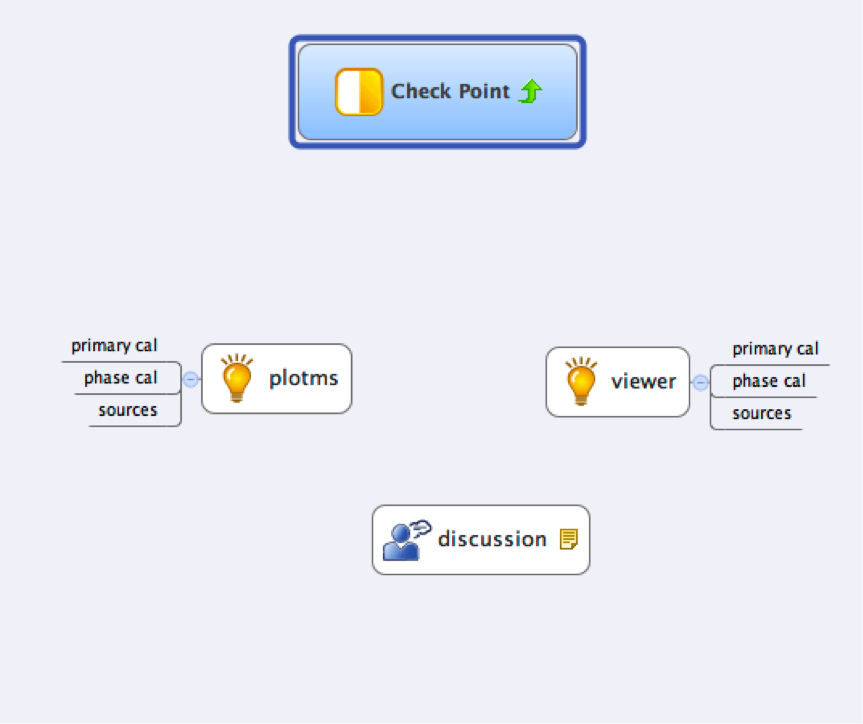
\includegraphics[width=12.0cm]{casa_flag.png}
%  \checkparity This is an \pageparity\ page.%
%  \caption[Mind map.]{}
%  \forceversofloat
%  \label{fig:casa_flag}
%  %\zsavepos{pos:textfig}
%\end{figure*}

The following tasks are available for flagging data in CASA:

\begin{itemize}
\item {\tt flagmanager}: save and manage versions of the flagging entries in the ms
\item {\tt flagautocorr}: noninteractive flagging of auto-correlations
\item {\tt plotms}: interactive XY plotting and flagging of visibility data
\item {\tt plotxy}: interactive XY plotting and flagging of visibility data -
note that plotxy is slower than plotms and will eventually be phased out
\item {\tt viewer}: can display (as a raster image) ms data, with some editing capabilities
\item {\tt flagdata}: This is the new non-interactive flagging (and
  unflagging) of specified data in CASA 3.4 onwards. It has other
  flagging options such as antenna shadowing, elevation flagging, etc.
%   Note that in future releases of CASA, this task will likely be
%   renamed just {\tt flagdata} and replace the older task of that name which
%   is still available the current (3.4.0) release of CASA.
\end{itemize}

We will mostly use the task {\tt plotms} to examine the data.  It is a very flexible tool that allows
you to interactively plot your visibility data in a wide variety of ways.  We will use it to identify
the bad data. We will then use the task {\tt flagdata} to actually flag it.  Although data {\em can}
be flagged directly in {\tt plotms}, we suggest that it is better to actually identify which antennas,
baselines and times are responsible for bad data before flagging them until you have some experience.
Flagging data {\em only} on the basis of e.g., low visibility amplitude can lead to serious biases: if
you expect a flux density of 1~Jy and you flag all the visibilities outside the range 0.9 to 1.1 Jy,
you would likely find the remaining visibilities suggested a source of 1~Jy.  However, you're not
learning about the sky, you're learning about the flagging you already did!

Calibrator sources are much easier to flag than program sources, because we largely know what kind of
source they are, and therefore what to expect from the visibility measurements.  In particular,
calibrators are generally point-like, which means the true visibility amplitude is independent of
baseline (and of time), and the phase should be 0\arcdeg.  Unfortunately, all we have available at
this point is the {\em uncalibrated} visibilities.  However, for an instrument like KAT-7, where all
the dishes, and thus all the baselines have approximately equal sensitivity, even for the uncalibrated
data for a point-like source, we can say this: the (uncalibrated) visibility amplitude on all
baselines should be approximately the same, say within a factor of 2 or so, and the (uncalibrated)
visibility phases should be fairly stable, although they do not need to be near 0\arcdeg.

The two most common failures to identify are probably ``dead'' or malfunctioning antennas, and
channels which are corrupted by RFI, which is usually very narrow bandwidth.  Even though automatic
flagging has already been done by {\tt h5toms.py}, and may well have removed most of the strong RFI,
you should nonetheless always examine your data.

However, first let us remove some bits data which is known to be bad.  The KAT-7 correlator is known
to produce some visibilities with spurious amplitudes of exactly 0.  We will use {\tt flagdata} to
delete these.  We will also use a second invocation of the {\tt flagdata} to flag any data taken at
antenna elevations below 10\arcdeg.  Data taken at very low antenna elevations is often unreliable and
noisy, so unless much of your data is taken at low elevations, its often easier to just delete the
small fraction with antenna elevations below about 10\arcdeg.

\begin{casacmd}
\begin{verbatim}
flagdata(vis=msfile,mode='clip',field ='',
  clipzeros=True, flagbackup = False)

flagdata(vis=msfile,mode='elevation',
  lowerlimit=10.0, flagbackup=True) 
\end{verbatim}
Note that in ``elevation'' mode, the elevation limits provided are those of the {\em good} data,
rather than those of the data to be flagged, so in this case any data below an elevation of 10\arcdeg\
will be flagged.  We do not need to set an upper elevation limit.
\end{casacmd}

Now lets plot the remaining visibilities.  Phase stability, both in frequency and time, is probably
the most important thing to check first: unless the visibility phases for the calibrator sources are
reasonably stable in time and across the different channels, calibration will likely prove impossible.

Each visibility point is associated with one baseline, that is some {\em pair} of antennas.  However,
instrumental failures are almost always antenna-dependent, that is, due to a failure of some
particular antenna, and therefore {\em all} the baselines involving the bad antenna will have bad
visibility data.  When identifying data to flag, it is best to try first to establish whether it is
some antenna that is bad, and if so flag all the data to that antenna.  Some bad data, however, in
particular that due to RFI, may not be antenna-dependent, and may have to be flagged individually per
baseline.

For starters, let us look at the phase as a function of frequency on a per-baseline basis.  We will
start with just one example scan of our strongest calibrator, {\tt PKS 1934-638}, pick one scan from
the listing above, somewhere near the middle of the run.  In this case we will pick scan ID = 57,
occurring between times 17:01:16.3 and 17:03:01.3.

Before you carry on, do spend some time getting to know the GUI behind
{\tt plotms} and how to use it: \\
\mbox{\url{http://casaguides.nrao.edu/index.php?title=Data_flagging_with_plotms}}.
For axis definition in plotms check this link : \\
\url{http://casaguides.nrao.edu/index.php?title=What\%27s_the_difference_between_Antenna1_and_Antenna2\%3F_Axis_definitions_in_plotms}.
Now actually run plotms to bring up the plot window and get a first look at part of our visibility
data.  Note that the {\tt iteraxis='baseline'} tells {\tt plotms} to plot each baseline individually.
Pressing the green arrow at the bottom of the {\tt plotms} interface will allow you to step through
the individual baseline plots interactively.

\begin{casacmd}
\begin{verbatim}
plotms(vis=msfile, xaxis='channel', yaxis='phase',
  correlation='XX,YY', scan='57', field='PKS 1934-638',
  iteraxis='baseline', coloraxis = 'corr',
  plotrange=[0,0,-180,180])
\end{verbatim}
\end{casacmd}

Your screen will look similar to this:
\begin{figure*}
  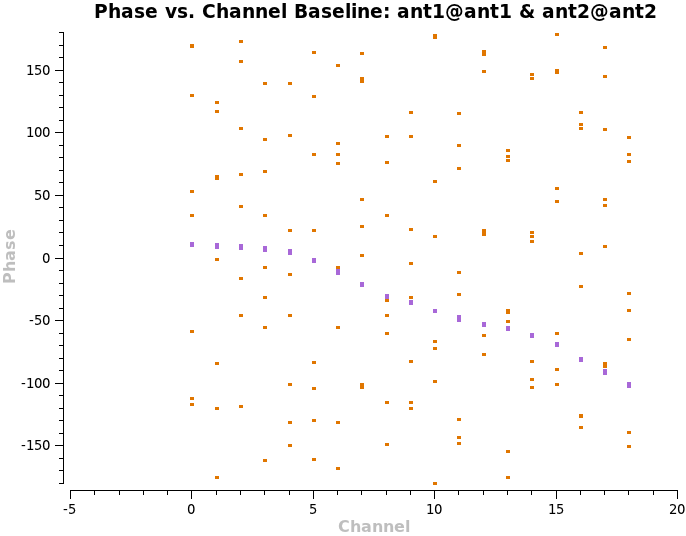
\includegraphics[width=10cm]{images/plotms_phas_v_channel_bl1}
%  \checkparity This is an \pageparity\ page.%
  \caption[Mind map.]{The output of plotms showing phase versus channel
for one baseline.}
  \forceversofloat
  \label{fig:plotms_amp_v_channel}
  %\zsavepos{pos:textfig}
\end{figure*}

The two different colours represent the two correlations or polarization products ({\tt XX,YY}) which
we have plotted.  Note that the purple points, which correspond to {\tt XX}, hang together well,
sloping slightly from channel 0 to channel 19.  They are fine.  The tan-coloured points for the other
polarization, however, are scattered randomly, and will not be usable.  This plot is for the baseline
between {\tt Ant1} and {\tt Ant2}.  Hitting the right arrow button at the bottom will show the plot
for the next baseline {\tt Ant1, Ant3}, where both polarizations look fine.  The next plot, {\tt Ant1,
Ant4} again shows the {\tt XX} points are fine, while the {\tt YY} points show strong variation across
the band.

These effects are almost certainly due to an {\em antenna}, rather than a single baseline, and the
trick is to identify which of the antennas is the one that is affected.  By stepping through the
baseline you will see that the {\tt YY} phases for all baselines involving {\tt ant2} look quite
random, while those involving {\tt ant4} are somewhat less random, but nonetheless show large
variation from channel to channel.  In other words, at least for this scan, there is a problem with
the phase stability for the {\tt YY} polarization of {\tt Ant2} and {\tt Ant4}.

Let us check for phase stability against time.  We will only plot one channel by specifying {\tt
spw='*:9'} for this purpose.  (Seeing as the phase will vary both with time and channel, its hard to
determine the phase stability by looking at all channels and times simultaneously, that's why we've
taken the approach of first taking a ``slice'' in time, and looking at only one scan but all channels.
Now we take a ``slice'' in frequency, and look at only one channel but at all times).

\begin{casacmd}
\begin{verbatim}
plotms(vis=msfile, xaxis='time', yaxis='phase',
  correlation='XX,YY', spw='*:9', field='PKS 1934-638',
  iteraxis='baseline', coloraxis = 'corr',
  plotrange=[0,0,-180,180])
\end{verbatim}
\end{casacmd}

Again you will see a similar pattern.  The visibility phases for {\tt XX} are quite stable in time,
showing only small variations from scan to scan and within each scan (mostly, the $\sim$10 or so
visibility points within a scan are so close together that the whole scan appears as a single point in
the plot).  However, again, the visibility phases for the {\tt YY} polarization (tan colour) for {\tt
ant2} and {\tt ant4} are quite unstable.

Since we have shown that the visibility phases for {\tt YY, ant2} and {\tt ant4} are quite unstable
both in time and across channels, we will delete these points.  Note, however, that so far, we have
only examined the data for one source, namely {\tt PKS 1934-638}.  Perhaps the data for the other
sources are fine!  Before throwing out all the data, its worth checking.  In the {\tt plotms} window,
change ``field'' to {\tt PKS 1613-586} and hit ``plot''.  There are more data for this source, but you
will see the exact same pattern.  Since the data for {\tt YY, ant2} and {\tt ant4} are bad for both
our calibrator sources, we have no choice but to flag all these data, including that for our target
source {\tt Circinus X-1}.  Very likely the target source data would also be bad, but in any case it
cannot be calibrated so we cannot use it.  You {\em could} plot also the visibility data for {\tt
Circinus X-1}, however since its not known to be a compact source we do not know what to expect from
the visibility phases.  They may vary strongly because the source is complex.  It is only for
calibrator sources, where the actually visibility phase should be constant that we can judge stability
by plotting the visibility phases as we have done.

At present CASA has the limitation that it cannot calibrate one of the {\tt XX, YY} polarizations when
the second one is missing, so we will actually have to flag all the polarizations for {\tt ant2} and
{\tt ant4}, even though the {\tt XX} polarization data does not have any problem.  (There are four
total correlations, {\tt XX, YY, XY, YX}.  We will deal only with first two, whose sum represents the
unpolarized intensity.  The calibration of the polarized parts, {\tt XY,YX} involves extra steps, and
is not yet implemented in CASA for linearly polarized feeds like those of KAT-7).  Having identified
the bad data, we once again turn to {\tt flagdata} to actually flag it.  We do not specify either {\tt
field} or {\tt correlation} so {\tt flagdata} flags the requested data for all fields and
correlations.

\begin{casacmd}
\begin{verbatim}
flagdata(vis=msfile, antenna='ant2,ant4',
  flagbackup=True)
\end{verbatim}
\end{casacmd}

\comment{
Referring to an antenna can be kind of confusing in CASA.  Like sources, CASA can refer to antennas by
their IDs or numbers, or by their names.  The confusing thing is that the antenna names often look
very similar to IDs, with KAT antennas having names like, e.g., ``ant1''.  However, the antenna IDs
start with 0, while the names start with the number 1.  You have to keep track of whether you are
referring to the antenna by ID or by name.  In this case, the antenna ID=0 has the name ``ant1'' (as
can be seen from the {\tt listobs} output).  So it is antennas {\tt ant2} and {\tt ant4}, also known
as {\tt ID = 1} and {\tt 3}, which have the bad data in this case.
}

If you now repeat the above {\tt plotms} commands, you will see that the visibility phases are now
nicely coherent for all the plotted baselines, and the baselines we have flagged no longer show up.

Now lets turn to the visibility amplitudes.  Again we make use of the fact that for continuum
calibrator sources, the expected values are known and should be the same on all baselines, and vary
only slightly across the channels.  This time we can plot all the baselines together, rather than
iterating through them as we did before:

\begin{casacmd}
\begin{verbatim}
plotms(vis=msfile, xaxis='channel', yaxis='amp',
  correlation='XX,YY', field='PKS 1934-638',
  coloraxis='corr')
\end{verbatim}
\end{casacmd}

You will see that for most channels there is only a relatively small variation of the visibility
amplitude with channel for PKS~1934-638 (note the amplitude scale on the left).  This small variation
will be corrected later with {\tt bandpass}.  However, channel {\tt ID=6} shows a much larger scatter
than any of the others, which is indicative that there may be RFI in this channel.  Switching to the
other calibrator source shows the same pattern.  It is sometimes diagnostic to also examine the {\tt
XY, YX} polarizations here.  For calibrator sources, we expect the polarized flux density to be a
relatively small fraction of the unpolarized (i.e., {\tt XX, YY}) one, whereas RFI is often strongly
polarized. We conclude that channel {\tt ID=6} is likely affected by RFI, and therefore we will
proceed to flag it also, once again using {\tt flagdata}.  Once again, we will flag that channel also
for the target source data, since even if the target source data were not also affected by the RFI,
the data would be uncalibratable.

\begin{casacmd}
\begin{verbatim}
flagdata(vis=msfile, spw='0:6', flagbackup=True)
\end{verbatim}
\end{casacmd}

We have now flagged most of the bad data affecting this run, in particular the bad data for the
calibrator sources, and can now proceed to the actual calibration.


\section{STEP 4... Calibration}

In order to explain calibration, we must first explain briefly the nature of the visibility
measurements we are trying to calibrate.  If the field of view is small enough so that it can be
represented as a plane (rather than as a curved part of the celestial sphere), then the sky brightness
can be written as $I(l,m)$, where $l$ and $m$ are the two orthogonal coordinates (typically RA and
decl).  The visibility function measured by an ideal interferometer, $V$, is given by a
two-dimensional Fourier transform of this sky brightness:

\begin{equation}
V(u,v)=\int\int I(l,m)e^{j2\pi(ul+vm)}dl dm
\end{equation}

where $u, v$ represent the coordinates in the Fourier transform plane.  At any given instant, each
baseline, or pair of telescopes, in the interferometer measures this visibility function at a point in
the Fourier transform plane whose $u, v$ coordinates are determined by the length and orientation of
the baseline, as projected onto the sky plane.  Since the telescopes rotate with the earth, each
baseline typically sweeps out an elliptical path in the $u, v$ plane as the earth rotates.  Although
$I$ is real, $V(u,v)$ is generally complex, with non-zero values for both real and imaginary parts.
$V(u,v)$ is often described as an amplitude and a phase, rather than by its real and complex parts.
Note that $V(u,v)$ is symmetric with $V(u,v) = V(-u,-v)$: generally the Fourier transform of a real
function, like $I$, is complex but symmetric.

The correlator output differs from the $V$ measured by an ideal interferometer for a variety of
reasons, to do with both instrumental effects as well as propagation effects in the earth's atmosphere
and ionosphere\footnote{At low frequencies, such as those observed by KAT-7, the effect of the
ionosphere is usually the dominant one}. The relationship between the observed and the true visibility
on the baseline between two telescopes, $i$ and $j$, can be written in a very general way as:

\begin{equation}
V_{ij}^{\rm observed}=J_{ij}V_{ij}^{\rm true}
\end{equation}

$J_{ij}$ represents the accumulation of all corruptions affecting the visibility measurement on
baseline $ij$.  Both $V$ and $J$ have complex values and are generally functions of frequency,
polarization and time, but we have suppressed the additional indices pertaining to frequency,
polarization and time for clarity.

Calibration involves determining the values of $J_{ij}$, in order to invert the above equation and to
determine the best approximation possible of $V_{ij}^{\rm true}$ from the observed values of
$V_{ij}^{\rm observed}$.

This task of determining $J_{ij}$ is made considerably easier by the fact that most of the effects
contained in $J_{ij}$ are {\em antenna}-based.  In other words, $J_{ij}$ can be factored into $J_i
\otimes J_j^*$ (where $J_j^*$ is the complex conjugate of $J_j$.  For an array consisting of $N_{\rm
ant}$ antennas there are therefore only $N_{\rm ant}$ unknown values of $J_i$ which need to be
determined, rather than the approximately $N_{\rm ant}^2$ values of $J_{ij}$ which would be required
otherwise.  Bear in mind that we have suppressed the time and frequency dependence here, so $J_i$ is
not a single complex number, but a function describing the complex response of antenna $i$ in both
time and frequency over the time-range and bandwidth of the observations.

The factorization occurs because the bulk of $J_{ij}$ has its origin in effects which corrupt the
radio signal as it travels through the atmosphere and the antenna electronics, these effects are
therefore due to an individual antenna $i$, but do not depend on the other antenna $j$ which makes up
that particular baseline.  Although there are baseline-dependent effects, they are mostly very small,
and for most purposes, can be ignored.

It is practical to further factor the $J_i$ into different components, representing different factors
affecting the radio signal, each of which can be determined independently.  Some of the components,
for example, are time-invariant, and therefore need to be determined only once for the observing run,
while others are time-variable.  In our calibration process, we will first factor $J_{ij}$ into the
antenna-dependent $J_i$ and thenceforth into a series of different factors, and each factor will be
determined in a different step.  Our approach is similar to the so-called ``Measurement Equation'',
which is a more formal approach to factoring $J_{ij}$ described in \citep{HamakerBS1999}, but we
factor $J_{ij}$ into slightly different components.

So we can write:

\begin{equation}
V_{ij}^{\rm observed} = J_{ij} V_{ij}^{\rm true}
                   = (J_i \otimes J_j^*) V_{ij}^{\rm true}
\end{equation}

where
\begin{equation}
J_i = A_i B_i G_i  \dots
\end{equation}

For example, $A_i$ might be corrections for some effect known a priori, such as an error in one of the
antenna positions used in the correlator, and $B_i$ might be to describe the bandpass response of the
antennas, in other words the variation in sensitivity and phase between the different channels, which
is taken to not vary with time, while $G_i$ provides the variation in amplitude and phase response as
a function of time, but taken not to be a function of frequency, i.e., determined for all frequency
channels simultaneously.  Note that the separation of these effects is not unique, however, we want to
ensure that the final product $J_i$ must be correct.

Some parts of $J_i$ can be calculated without any reference to the visibility data.  However, most of
$J_i$ will be determined from the values of $V^{\rm observed}$ for calibrator sources, where we know
what the values of $V^{\rm true}$ should be and can therefore invert the equation above.  In
particular, most of the parts of $J_i$ due to the atmosphere and ionosphere cannot be known in
advance.  The values of $J_i$ (recall that $J_i$ in general depend on time, but we have suppressed
this dependence in the notation), determined from the observations of calibrator sources are then
interpolated (or extrapolated) to the times corresponding to the observations of the intended target
source(s). The various calibration programs perform the function of estimating the antenna-based
calibration factors (e.g., $A_i, B_i$ etc., from above) from the (baseline-based) calibrator source
visibility measurements.

For example, the antenna-based bandpass response, $B_i$ is typically treated as being independent of
time (although it is by definition a function of observing frequency).  It is typically determined by
examining the visibilities for a strong calibrator source of known spectrum (the simplest case would
be a source with a flat spectrum, with true flux density independent of the particular frequency or
channel under consideration).  Often this is the first step in the calibration, since once this
bandpass correction is known, we can use an average across the channels to determine the remaining
parts of $J_i$, rather than having to do it for each channel independently.

In order to use the visibility data from calibrator sources to calculate calibration quantities, such
as the bandpass response, one should edit out the bad visibility data first.  This is why we started
above with examining the data and flagging bad points or antennas.

The typical sequence is to first use observations of a strong calibrator, often the flux-density
calibrator, to determine the bandpass response.  With that in hand, we no longer have to make separate
solutions for every channel, but can combine them.  One then uses the observations of calibrator
sources to determine the variation of $J_i$ with time.  Many calibrator sources are variable on
timescales of weeks or longer and their flux densities are therefore not accurately known.  In order
to set the flux density scale correctly, one needs observations of at least one flux density
calibrator source, whose flux density {\em is} known. Typically, one uses one or a few scans of a flux
density calibrator source for this purpose, and then the remainder of the $J_i$ can be obtained from
other calibrator sources whose flux density is not known (although it should not vary during the
observing run), but which {\em are} known to be point-like.  These secondary calibrators are known as
phase calibrators or secondary amplitude calibrators.

So, lets begin the calibration. For safety and sanity, one should begin by ``clearing the
calibration''.  The data structure of CASA measurement sets (ms) is that the observed data are stored
in a {\tt DATA} column of the ms, while the corrected data (i.e., those multiplied by $J_{ij}$) are
stored in the {\tt CORRECTED\_DATA} column once they become available.  The values from which $J_{ij}$
are constructed are stored in various calibration tables.  There is a further column of visibility
data called {\tt MODEL\_DATA} where model values, if available, such as the expected visibility values
for a calibrator of known structure, are stored.  The task {\tt clearcal} initializes the {\tt
CORRECTED\_DATA} and {\tt MODEL\_DATA} columns and therefore clears calibrated data from any previous
attempts at calibration from them.

\begin{casacmd}
\begin{verbatim}
  clearcal(vis=msfile,field='')
\end{verbatim}
\end{casacmd}

\begin{figure*}
  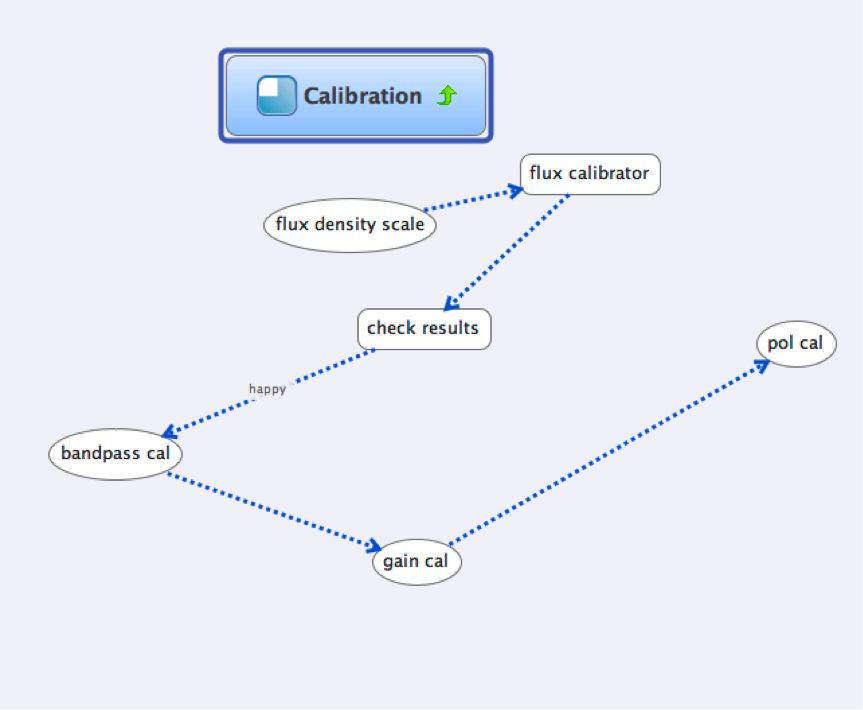
\includegraphics[width=10.0cm]{images/casa_cal}
%  \checkparity This is an \pageparity\ page.%
  \caption[Mind map.]{A schematic diagram of the calibration process.}
  \label{fig:textfig}
  %\zsavepos{pos:textfig}
\end{figure*}

\bigskip
\pause{ Time to take a break and have some coffee... The steps after will need more attention.}

% \medskip
\bigskip

There are few sources whose flux density is known reliably which can be used as primary amplitude
calibrators.  The task {\tt setjy} knows about the most common of these, and will insert the correct
flux density for the frequency of the observations as well as entering the model into the {\tt
MODEL\_DATA} column for subsequent use.

\caution{
These primary flux density calibrators are often somewhat resolved, and thus source models should be
used to represent the source structure.  The task {\tt setjy} can be invoked to list the available
source models (with {\tt listmodels=True}).  However, the flux density calibrator for our observations
is {\tt PKS~1939-638}, which is one that is close to ideal in that it has no structure on scales
larger than 1\arcsec.  The default point model is therefore adequate and no further source model is
required in our case.
}

We still have to enter the actual flux density for {\tt PKS~1939-638} for the actual frequency of the
observations.  In general the flux density varies with frequency, and {\tt setjy} will calculate a
slightly different value for each channel from the known spectrum.  (In the case that a model image is
used for the flux-density calibrator, {\tt setjy} will also scale the model image to the total flux
density for each channel in the ms, and then enter the Fourier transform of the scaled model image
into the MODEL\_DATA column for that source and channel.) Setting {\tt fluxdensity = -1} causes {\tt
setjy} to look up the flux density for flux density calibrators and enter the standard value.

%1934 - 4.2mas double

\begin{casacmd}
\begin{verbatim}
setjy(vis=msfile, field='PKS 1934-638',
      scalebychan=True, standard='Perley-Butler 2010',
      fluxdensity=-1)
\end{verbatim}
\end{casacmd}

\medskip
{\tt setjy} should produce the following output in the logger, from which one can see that it has
identified calibrator source {\tt PKS~1934-638} and filled in the known flux density of $\sim$13~Jy in
I (the exact flux density will vary somewhat and be slightly different in the different channels, with
the listed value being that for the channel at the reference frequency of 1932~MHz).  If you see the
message that your source ``{\tt is not recognized by Perley-Butler 2010}'', then {\tt setjy} will have
entered a default flux density of 1.0 Jy for your flux calibrator and you have to fix the problem
otherwise your flux density scale could be wrong by a large factor.
%MFB:  I have taken out mention of the VLA calibrator manual as
%MFB:  1934-638 does not seem to be in there!

% %  for CirX1.ms
\begin{casaoutput}
\begin{verbatim}
setjy::::casa	##### Begin Task: setjy              #####
......
setjy::imager::setjy()	Using channel dependent flux densities
setjy::imager::data selection	Selected 2709 out of 71904 rows.
setjy::imager::setjy()	PKS 1934-638 (fld ind 0) spw 0  [I=13.182, Q=0, U=0, V=0] Jy, (Perley-Butler 2010)
....
\end{verbatim}
\end{casaoutput}

\medskip
Once we are happy that the correct flux density has been entered for the flux-density calibrator, we
can proceed to the next step, which is to solve for the bandpass response, in other words for the
variation of the complex antenna gains across the different channels.  (Note that {\tt setjy} above
did not yet solve for any part of $J_i$, it only entered the flux density of our calibrator,
essentially the value of $V^{\rm true}$ into the ms so that we {\em can} start solving for $J_i$ in
the next steps.  The variation of the gains across the observing band is largely due to instrumental
effects and usually quite stable, so we only need to solve for it once.  Once we have solved for the
bandpass response, we can combine all the channels in a single solution for the subsequent steps.

However, we have the problem that the phase part of $J_i$ can be quite rapidly time-variable even
though the amplitude part is not.  In order to properly calculate the bandpass response, we therefore
want to do some temporary phase-calibration for that scan which we intend to use for the bandpass
calibration, to prevent decorrelation when vector averaging the data in computing the bandpass
solutions.  In other words, to obtain the bandpass solution, we will average the complex visibility
data in time over a whole scan.  If there is any variation on phase over the scan, we want to
calibrate that out before performing the bandpass solution.

We do this phase calibration using {\tt gaincal}, and using only a portion of the band, in this case
the six channels from 7 to 11.  These solutions for the antenna phases as a function of time can then
be used to calibrate out any variation in the phase during the scan for the purposes of the subsequent
bandpass solution.  The rapid phase variation we are calibrating out here are due mostly to the
atmosphere, and are not expected to vary significantly between the channels.  Therefore, although
these phase solutions are determined from only a central portion of the band, they are applicable to
the whole band (i.e., to all 19 channels).  The choice of the particular channels (7 to 11) is
relatively arbitrary, but usually its best to use a few channels near the centre of the band, which
were found to be relatively free from interference in the editing steps earlier.

For this next step, we need to specify a reference antenna.  When we ran {\tt h5toms} we chose
reference antenna 5.  However, its possible that antenna 5 was not present at all during the run, or
that we removed some of its data in flagging.  You can use {\tt plotms} to plot {\tt antenna1} against
{\tt time} for all fields to quickly identify which antennas were present during which parts of the
run.  In this case you should see that antenna ID=0 is missing during the first part of the run,
because we flagged it earlier.  Antenna ID=5 seems to be present throughout, and can therefore serve
as our reference antenna for the rest of the calibration.  Note that it is possible to use different
reference antennas for different parts of the calibration, but if possible you should use the same
antenna throughout.  It is also desirable to choose a reference antenna which is known to be stable
and fairly sensitive (in the case of KAT-7 the sensitivities of the 7 antennas is very similar, so the
only real criterion for picking the reference antenna is stability).

\begin{casacmd}
\begin{verbatim}
gaincal(vis=msfile, caltable=gain_table0,
  field='PKS 1934-638', refant=reference_antenna,
  spw='0:7~11', calmode='p', solint='int',
  minsnr=4, minblperant=4, solnorm=T, gaintable='')
\end{verbatim}
Remember that we defined the variables {\tt refant} and {\tt gain\_table0} earlier to hold the name of
the reference antenna and gain table, respectively, that we're using for this particular ms.
\end{casacmd}
%MFB: i've changed minsnr to 4 here, if we're getting SNR<3
%MFB: on this for some vis, we're probably better off just
%MFB: not using them for bandpass calibration;  I've also
%MFB: just arbitrarily picked channels 7~11

After having determined the solutions, we should examine them using {\tt plotcal}. The task {\tt
plotcal} can plot a variety of gain solutions in a variety of ways, check {\tt help plotcal} to find
out more.  We remind you that {\tt gaincal} has factored $J_{ij}$ into antenna-based components, so
you don't see a set of values for each baseline, but rather only one for each antenna ($J_i$), and the
CASA programs will calculate the full value of $J_{ij}$ as needed when calibrating the visibility
values.

\begin{casacmd}
\begin{verbatim}
plotcal(caltable=gain_table0, xaxis='time',
  yaxis='phase', field='PKS 1934-638',
  iteration='antenna',  plotrange=[0,0,-180,180])
\end{verbatim}
\end{casacmd}

On the {\tt plotcal} plot, you should see that the gain-table phases (antenna phases, or the
phase-component to $J_i$) should be fairly stable during the minute or two of the scan-length.  Small
variations are fine, indeed the point of running {\tt gaincal} was exactly to find these small
variations so that they can subsequently be calibrated out from the visibilities.  However, if the
antenna phase appears random from one point to the next then something has likely gone wrong.

Now we can run {\tt bandpass} to solve for the complex gain as a function of channel across the
observing band.  Specifying {\tt gaintable=[gain\_table0]} causes bandpass to apply the time-dependent
antenna phase calibration we determined in the previous step before forming the bandpass solutions.

\begin{casacmd}
\begin{verbatim}
bandpass(vis=msfile, caltable=bandpass_table0,
  field='PKS 1934-638', refant=reference_antenna,
  solnorm=True, combine='scan', solint='inf',
  bandtype='B', gaintable=[gain_table0])
\end{verbatim}
\end{casacmd}

You will see the message:
\begin{verbatim}
Insufficient unflagged antennas to proceed with this solve.
   (time=2012/07/01/22:08:07.6 field=0 spw=0 chan=6)
\end{verbatim}

Since we flagged channel 6 or {\tt spw=0:6} earlier on, this is not something to worry about, its just
telling us that there is no solution for that particular channel, but that doesn't matter because we
have no visibility left for that channel.  A message like this about some channel for which there {\em
was} visibility data left would be a problem.

The task {\tt plotcal} can also be used to display the bandpass solution:

\begin{casacmd}
\begin{verbatim}
plotcal(caltable=bandpass_table0, xaxis='chan',
  yaxis='amp', subplot=222, iteration='antenna')
\end{verbatim}
\end{casacmd}
%  hmm, there only seem to be solutions for some antennas
%  no solns for ant2 or ant4;  strangeness: plotcal plots
%  ant1-6, then leaves ant2-6 plots up but replaces
%  ant1 plot with ant7 one!
%   It does not get a solution for ant2,4
%  aha- ant2-4 have no data for the longer flux-cal scan
%   at end; neither of these antennas have any data for
%   1939!

First note that plots for the antennas for which the data have been flagged ({\tt ant2, ant4}) are
blank, which is as expected.  For the others the gain amplitude varies only by 10\% to 20\% across the
channels, which is in the expected range.  Since we asked {\tt bandpass} to normalize the solution,
the average gain for each antenna is 1.0 --- at this point we're only after the variation across the
band.  If any of the gains were to differ from unity by more than a factor of 2 or so, then may be
more bad data to flag.  One would then have to flag that bad data, and then re-start the calibrations
from the {\tt clearcal()} step.

The next step derive the main, time-variable, part of $J_i$, which we term $G_i$.  This is done for
each source individually, by comparing the observed visibilities $V_{ij}^{\rm observed}$ to the
expected visibilities $V_{ij}^{\rm true}$.  For the flux density calibrator, we have determined the
latter values, and we can get the correct values for $G_i$.  For the phase calibrator sources, we
assume a point source model, so we know the phase part of all the $V_{\rm true}$ is 0.  We {\em
assume} for now that the unknown flux-density of the phase-calibrator sources is exactly 1.0 Jy
(typically they are of this order). If we then solve for $G_i$, we will obtain complex values whose
amplitudes differ from the correct ones by a factor depending only on the true source flux density (by
([1 Jy]/[true source flux density])$^{0.5}$).  We can then compare the $G_i$ obtained for the
secondary calibrators, and scale them so that they match as well as possible the correctly-scaled
amplitudes of $G_i$ obtained for the primary flux-density calibrator.  The scaling required gives us
the true flux density of the secondary calibrator source in terms of the originally assumed one, i.e.,
1 Jy.  This process is known as ``flux density bootstrapping''.

The reason for this complicated procedure is that there are only a handful of flux-density
calibrators, so it is generally impossible to choose a flux density calibrator close to the target
source on the sky.  There are many phase calibrator sources, however, so a phase calibrator can be
chosen that is much closer on the sky (typically a few degrees~\arcdeg\ away).  The flux density
bootstrapping allows us to use the phase and amplitude calibration (i.e. $G_i$) from these much nearer
calibrator sources, which will provide a much better calibration for the target source, but to set the
flux density scale accurately from observations of the flux density calibrator.  The flux density
scale is usually stable for hours, so once we have transferred the flux density scale to the phase
calibrator sources by flux density bootstrapping, the solutions we obtain for the phase calibrator
sources are equivalent to those which would have been obtained if we'd known the flux density of the
phase-calibrators to begin with.

First we determine the values of $G_i$, also called the complex gains, for the flux-density
calibrator:

\begin{casacmd}
\begin{verbatim}
gaincal(vis=msfile, caltable=gain_table1,
  field='PKS 1934-638', solint='inf',
  refant=reference_antenna, gaintype='G',
  calmode='ap', gaintable=[bandpass_table0])
\end{verbatim}
Note that the a new solution is started for each scan, the {\tt solint='inf'} only means that the
solution interval can be arbitrarily long {\em up to} the next scan boundary.
\end{casacmd}

Next we determine the complex gains for the phase calibrator (so far under the assumption that it has
a flux density of 1~Jy).

\begin{casacmd}
\begin{verbatim}
gaincal(vis=msfile, caltable=gain_table1,
  field='PKS 1613-586', solint='inf',
  refant=reference_antenna, gaintype='G', calmode='ap',
  append=True, gaintable=[bandpass_table0])
\end{verbatim}
Note that the {\tt append=True} causes {\tt gaincal} to append to the specified gain table, rather
than over-writing it.
\end{casacmd}

Plotting again to have a look at the solutions:

\begin{casacmd}
\begin{verbatim}
plotcal(caltable=gain_table1, xaxis='time',
  yaxis='amp', iteration ='antenna')
\end{verbatim}
\end{casacmd}

Notice that, for each antenna, there are two sets of points.  The lower set, in this case with gain
amplitudes near $\sim$0.1 corresponds to our flux density calibrator ({\tt PKS 1934-638}).  Since we
were working with the correct flux density for this source ($\sim$13 Jy), these gains already have the
correct values.  The other set of points, with values near $\sim$0.2, are those for {\tt PKS
1613-586}, which differ from the true values by a scale factor.  The next step is to derive this scale
factor, so as to make the two sets of points match as well as possible.  The true flux density of {\tt
PKS 1613-586} can be trivially determined from the derived scale factor.

The task {\tt fluxscale} calculates the scale factor, thus performing the bootstrapping, and will
output a correctly scaled version of the calibration table, which we can then use to calibrate the
data, as well as printing out the derived value for {\tt PKS 1613-586}'s flux density.

\begin{casacmd}
\begin{verbatim}
fluxscale(vis=msfile, caltable=gain_table1,
  fluxtable=flux_table1, reference=['PKS 1934-638'],
  transfer=['PKS 1613-586'])
\end{verbatim}
\end{casacmd}

\begin{casaoutput}
\begin{verbatim}
INFO fluxscale	##### Begin Task: fluxscale          #####
INFO fluxscale	Opening MS: CirX1.ms for calibration.
INFO fluxscale	Initializing nominal selection to the whole MS.
INFO fluxscale	Beginning fluxscale--(MSSelection version)-------
INFO fluxscale	 Found reference field(s): PKS 1934-638
INFO fluxscale	 Found transfer field(s):  PKS 1613-586
INFO fluxscale	 Flux density for PKS 1613-586 in SpW=0 is: 4.6868 +/- 0.012777 (SNR = 366.816, N = 10)
INFO fluxscale	Storing result in CirX1_spw0.fluxscale1
\end{verbatim}
\end{casaoutput}

% \bigskip
{\bf What is it we can deduce from this output? How do we know everything is fine?}  First, we can
examine the messages produced by {\tt fluxscale}.  It has determined a flux density for {\tt PKS
1613-586} of $4.687 \pm 0.013$~Jy, making it a fairly strong source.  For a strong source like this,
the uncertainty in the bootstrapped flux density should be $<1$\%, which indeed it is.  You can also
check that the flux density is within the range of values usually seen for your particular source at
this frequency.  For example, our source, {\tt PKS 1613-586}, is listed in the ATCA calibrator list at
(\url{http://www.narrabri.atnf.csiro.au/calibrators}) as having flux density of 4.21~Jy at 1.75~GHz
(the closest of the listed frequencies to ours), so our value of 4.687~Jy is quite reasonable, as its
only 16\% higher.  Variations of a factor of 2 are not uncommon, if you get a flux density more than a
factor of 2 different than the listed, you may want to double check.

If you use {\tt plotcal} as above, but on the new version of the table produced by {\tt fluxscale},
i.e. {\tt caltable=flux\_table1}), you will see that the gain amplitudes for {\tt PKS 1913-638} are no
longer readily distinguishable from those for {\tt PKS 1613-586}, which was the goal (the gain of the
antennas should not depend on which source you are observing!).  You may also plot the gain phases
with:

\begin{casacmd}
\begin{verbatim}
plotcal(caltable=flux_table1, xaxis='time',
    yaxis='phase', iteration ='antenna',
    plotrange=[0,0,-180,180])
\end{verbatim}
\end{casacmd}

And you should see that the gain phases are in fact very stable in time, and relatively consistent
between our two calibrator sources.  For {\tt ant5} the gain phases will be exactly 0\arcdeg\ as this
was our reference antenna, so it has a gain phase of 0\arcdeg\ by definition.  In order to calibrate
the visibility data for our target source, we have to interpolate between the calibrator gain values.
Since the gain phases for our phase calibrator source {\tt PKS 1613-586} form a nice smooth line (in
fact the individual points may not be distinguishable on your plot), the interpolation should yield an
accurate value. If, on the other hand, the gain phases (or amplitudes) differ drastically from one
point to the next, then interpolation to the intervening target-source observations will be dubious.

Our calibration therefore is looking good.  The next step is to actually use it to calibrate the
visibility data and produce our estimates of $V_{ij}^{\rm true}$.  Here is where we calculate the
$V_{ij}^{\rm true} = V_{ij}^{\rm observed} J_{ij}^{-1}$.  This is where we want to be careful about
how we interpolate our gain solutions ($J_i$).  For example, on the plot of gain phase against time,
you could see the gain phases for {\tt PKS 1613-586} all lay on a fairly smooth curve, while those for
{\tt PKS 1934-638} did not quite lie on the curve.  Since {\tt PKS 1613-586} is much closer on the sky
to our target source ({\tt Circinus X-1}) the gain values (i.e., values of $J_i$) derived from {\tt
PKS 1613-586} are better for interpolating to the target.  However, we also want to calibrate the
visibility data for {\tt PKS 1934-638}, and of course here we're much better of using the gain
solutions derived from {\tt PKS 1934-638} itself.  (Note that although at this point, we're largely
done with our calibrator sources, and will not have any immediate further use for the
calibrator-source visibilities, its probably a good idea to apply the calibration properly to the
calibrator sources as well as the target source).

The easiest way to keep it straight is to apply the calibration separately to each source.  The task
that applies the calibration is called {\tt applycal}.  It combines the requested gain tables,
interpolates or extrapolates as required to determine the full antenna-based $J_i$, calculates the
baseline-based $J_{ij}$ values as needed for each visibility measurement, and then writes out the
properly calibrated visibility data (our estimate of $V_{ij}^{\rm true}$) into the {\tt
CORRECTED\_DATA} column of the ms.  You can specify the {\tt field}, which determines which source's
visibility data get corrected, and {\tt gainfield}, which specifies from which source's gain table
entries the required correction is determined.  The best calibration is usually when the {\tt field}
entry is the same as the {\tt gainfield} entry, but usually one does not have calibration solutions
for the target sources, so for the target source, {\tt gainfield} must necessarily be different than
{\tt field}.  Note that as {\tt applycal} can simultaneously apply several calibration tables, {\tt
gainfield} can have multiple entries, one for each calibration table to be applied.  The two
calibration tables we want to apply are the bandpass table, {\tt bandpass\_table0}, and the gain table
with the correct flux density scaling for {\tt PKS 1613-586} or {\tt flux\_table1}.  Since there are
two tables to apply, we need two entries in {\tt gainfield}.

Lets just start with the first source: {\tt PKS 1934-638}.  We want to calibrate its visibility data
and therefore set {\tt field} to {\tt PKS 1934-638}.  Since the {\tt bandpass\_table0} contains only
entries for {\tt PKS 1934-638} anyway, there is no choice and we can just leave the corresponding {\tt
gainfield} entry blank -- this will apply all sources in the table.  For the {\tt flux\_table}, we
want to use only the entries derived from {\tt PKS 1934-638} itself, so the second {\tt gain\_field}
entry should be {\tt PKS 1934-638}.  The parameter {\tt interp} specifies the nature of the
interpolation used in gain table in a manner analogous to {\tt gainfield} (see {\tt help applycal} for
details).  In this case we will just choose the entry nearest in time to the particular visibility to
be calibrated in {\tt bandpass\_table0} and interpolate linearly in {\tt flux\_table1}.

\begin{casacmd}
\begin{verbatim}
applycal(vis=msfile,
  gaintable=[bandpass_table0,flux_table1],
  field='PKS 1934-638',
  gainfield=['', 'PKS 1934-638'],
  interp=['nearest',''])
\end{verbatim}
\end{casacmd}

Next we turn to our phase calibrator.  {\tt field} should now be set to {\tt PKS 1613-586}.  Again we
can leave the first entry in {\tt gainfield} blank, since we again want to use any solutions in the
bandpass table.  However, this time we want the second {\tt gainfield} entry to be {\tt PKS 1613-586}.

\begin{casacmd}
\begin{verbatim}
applycal(vis=msfile,
  gaintable=[bandpass_table0,flux_table1],
  field='PKS 1613-586',
  gainfield=['', 'PKS 1613-586'], 
  interp=['nearest',''])
\end{verbatim}
\end{casacmd}

Finally, we apply the calibration to the target field.  Now {\tt field} becomes {\tt Circinus X-1}.
The first entry of {\tt gainfield} again can stay blank (we're again using the bandpass solution from
{\tt PKS 1934-634}).  For the second entry in {\tt gainfield}, however, we cannot use the same value
as {\tt field} like we did above, because we have no gain solutions for {\tt Circinus X-1}.  Since
{\tt PKS 1613-586} is much closer on the sky, we want to use its entries from {\tt flux\_table1}, but
not those from {\tt PKS 1934-634}, so the second {\tt gainfield} entry should again be {\tt PKS
1934-634}.

\begin{casacmd}
\begin{verbatim}
applycal(vis=msfile,
  gaintable=[bandpass_table0,flux_table1],
  field='Circinus X-1',
  gainfield=['','PKS 1613-586'],
  interp=['nearest',''])
\end{verbatim}
\end{casacmd}


\section{STEP 5... Splitting the data}

We are now almost ready to split the calibrated visibility data for our target source into separate ms
file.  Note that this step is convenient, rather than necessary.  One could just as well make images
(and even proceed to self-calibration) using the original ms, but often it is convenient to split out
the data of interest at this point.  This particular data set has already been averaged in frequency
to reduce the size for the purposes of the workshop.  These days most raw data sets you encounter will
likely have far more than 19 channels, and data sets from interferometers with more telescopes than
KAT-7, such as JVLA, ALMA, LOFAR and MeerKAT once it comes online, will have far more visibility
measurements at each time-stamp.  In such cases one might average down in frequency to reduce the size
of the data set and make for faster processing.  It is not necessary in this case, so our {\tt split}
output file will have the same number of channels as our original ms.

However, {\em before} you do any averaging, it is a good idea to briefly examine the calibrated
visibility data for the target source in case there is more bad data we need to flag.  Recall that so
far we have only examined the data for our calibrator sources, but not yet that for {\tt Circinus
X-1}.  Lets turn again to {\tt plotms}.  We will now plot correlated flux density against baseline
length in wavelengths ({\tt uvwave}).  Such plots are commonly made to diagnose the nature of the
source structure.  We now have to specify that we want the {\tt CORRECTED\_DATA} column: we've gone to
all this trouble to determine how to calibrate our visibilities, so we want to make sure we're
enjoying the fruits of our labours.

\begin{casacmd}
\begin{verbatim}
plotms(vis=msfile,  field='Circinus X-1',
  xaxis='uvwave', yaxis='amp',
  correlation='XX,YY', ydatacolumn='corrected',
  coloraxis = 'corr')
\end{verbatim}
\end{casacmd}

You should see something like this:
\begin{figure*}
  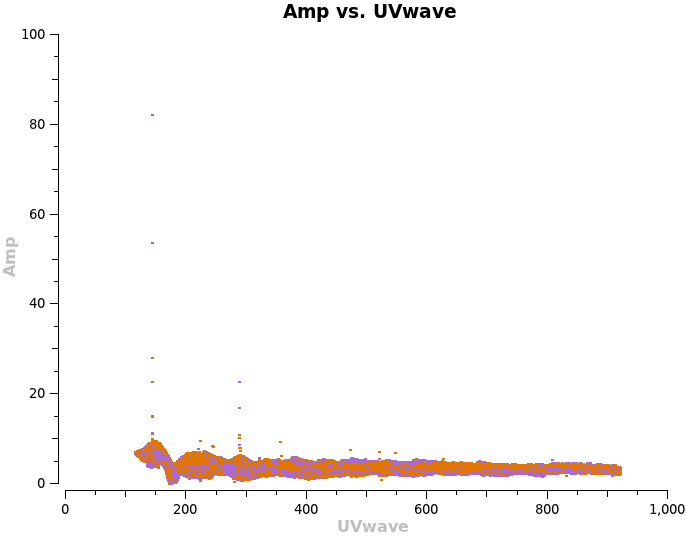
\includegraphics[width=10cm]{images/CirX1_uvplot}
%  \checkparity This is an \pageparity\ page.%
  \caption[Mind map.]{Plot of visibility amplitude against
    baseline-length for our target source, {\tt Circinus X-1}.}
  \forceversofloat
  \label{fig:CygX1_upvlot}
  %\zsavepos{pos:textfig}
\end{figure*}

This plot mostly shows that {\tt Circinus X-1} is {\em not} a point source, since the correlated flux
density seems to vary systematically with baseline-length ($uv$-distance or {\tt uvwave}).  There are,
however, a few outlier points still, with anomalously high amplitudes above 10~Jy, such as the spikes
at UVwave $\sim 140, 290 \, \lambda$.  These are likely due to RFI\@.  If we re-plot amplitude against
channel, you will see that all the high amplitude point are in a single channel: channel 18.  To
further narrow it down, select {\tt spw = '*:18'} and {\tt xaxis='time'}.  Not only do the
high-amplitude points occur in one channel, they occur at a specific time: near 25:40.  By zooming in
on the plot using the ``zoom'' tool (select the magnifying glass icon, and use the mouse to draw a box
on the screen showing the region you want to zoom in on.  You can zoom back out using the ``plot''
button), to see that the bad data occurs between times of 25:32:30 and the end of the scan at
25:34:00.  Although it is possible to flag graphically directly in {\tt plotms}, I encourage you to
again use {\tt flagdata}.  Firstly, it is better to positively identify the bad data to be flagged
first, rather than zapping points at random on the screen.  Secondly, using the {\tt flagdata} command
means that you can, if needed, precisely and accurately repeat the operation.  Note also, that we
could do more work to locate the bad data, it might for example be only one antenna or baseline which
is bad.  However, since its such a small amount of data (under 1.5 minutes in one channel only), its
more expedient just to flag it all.  Note also that {\tt plotms} labels time axes in a slightly
non-standard way with hours having values $>24$.  For {\tt flagdata} these values have to be
translated into a more formal timerange.

\begin{casacmd}
\begin{verbatim}
flagdata(vis=msfile,
  timerange='2012/07/02/01:32:30~2012/07/02/01:34:00',
  field='Circinus X-1', spw='0:18', flagbackup=True)
\end{verbatim}
\end{casacmd}

So now we've removed those outliers, we can split the data for our source of interest, {\tt Circinus
X-1}.

\begin{casacmd}
\begin{verbatim}
split(vis=msfile, outputvis='CirX1_split.ms',
  datacolumn='corrected',  field='Circinus X-1')
\end{verbatim}
\end{casacmd}


\section{STEP 6... CLEAN aka Deconvolution}

For interferometric data, the $(u,v)$ coverage is virtually never complete, and therefore the
instrumental response, called the dirty beam or the point spread function, PSF, has some unwanted
secondary responses, known as side lobes.  The Fourier transform of the visibilities represents the
convolution of the true image with the dirty beam.

There are various techniques to reduce the effects of the sidelobes, in other words to effect a
deconvolution.  In radio astronomy, deconvolution has been dominated by two non-linear algorithms:
CLEAN and the Maximum Entropy Method (MEM).

The original formulation of CLEAN was by \citet{Hogbom1974}, and worked purely in the image plane.  We
explain this method here as it is easier to understand.  Most modern implementations of CLEAN actually
work partly in the $(u,v)$ plane to produce somewhat more accurate results than H\"{o}gbom's original
image-plane formulation, but are conceptually similar.  CLEAN works iteratively, transferring flux
density from the dirty image to a set of point-like ``clean components'', which represent the true
distribution of emission on the sky or the deconvolved image.  After each step, a residual image is
formed which represents the original dirty image after subtraction of the CLEAN components so far.
Initially, before the first CLEAN component is found and subtracted, the residual image is just the
dirty image.

The H\"{o}gbom CLEAN algorithm proceeds using these steps:
\begin{enumerate}

\item Find strength and position of the brightest point in the current residual image.  CLEAN makes
the plausible assumption that this peak is mainly due to a real signal and only a minor part comes
from the sidelobe responses to other real emission farther away in the image.  Note that one should
specify one or more ``clean windows'' in which to search for real emission.
\item Subtract a point source at this location.  The brightness of the point source is taken to be the
brightness of the brightest point multiplied by a factor $\gamma (\leq 1)$ called the loop gain.  This
point source is the CLEAN component, and it is added to the list of CLEAN components.  The response of
the instrument to a point source is the dirty beam pattern.  Therefore, to subtract this point source
from our dirty image, CLEAN subtracts a dirty beam pattern, scaled so that its peak is the same as
that of the point source, and centred on the location of the brightest point, from the current
residual image.
\item Go to step 1 unless any remaining point sources are below some level specified for convergence,
or the maximum number of CLEAN components is reached.
\item Convolve the accumulated CLEAN components, which represent the model of the deconvolved
emission, with an idealized ``clean'' beam (usually an elliptical Gaussian fitted to the central lobe
of the dirty beam).
\item Add the final residual image to the convolution from the previous step.  The result is what is
called the CLEAN image.  Note that for purposes of calibration, it is usually the CLEAN components
that are used rather than the CLEAN image.

\end{enumerate}

The CLEAN algorithm was designed for the case where the true brightness distribution contains only a
few unresolved sources.  It works well for cases where the true emission occurs only within small,
well-separated, regions across the field of view, in other words if the field of view is {\em mostly}
empty.  The following excerpt has been taken from Robert Reid's Thesis \citep{Reid2003}.  ``Physics
and filled aperture measurements give us several properties that images should have. Non-negativity:
Astronomical objects, even black holes, cannot steal light away from our receivers, but raw
interferometric images abound with negative patches. Requiring the image to be non-negative is a
strong constraint on what should be used to fill in the gaps.  Locality: Usually the range of
directions from which light can be received is limited by the antennas being used. The rough location
and extent of the source may also be known from observations at other wavelengths. Raw images always
have ripples going off to infinity that should be quenched. If nowhere else, nulls in the antenna
reception pattern are invalid places to receive light from. For many frequencies and parts of the sky,
bright radio sources are also quite rare and confined (as known from filled aperture measurements), so
images are expected be mostly empty.  Smoothness: Sources are expected to be continuous, and usually
to have continuous derivatives. Also, it is best to minimize the effect of the unmeasured part of the
sampling plane on the final image. Perfectly sharp edges depend on the entire sampling plane, far
beyond where interferometers can make measurements. Smoothing the image concentrates its region of
dependence on the finite area that interferometers sample.  Agreement with theory: At first this seems
to throw out the baby with the bathwater, since true discoveries must be novel. True discoveries,
however, must rest on true observations. Since deconvolution ideally agrees with all the measurements,
we should not let non-measurements mislead us. Another way to see this is to think of the model as
assisting us in separating reasonable interpolations from unreasonable ones for the image, but the
parameters of the model itself are determined by the measurements. For example a circle has an
infinite number of points on its circumference, but three points on its locus are enough to specify
it, if we are sure that it is a circle. In any case, images tend to be constructed before models, thus
this principle is not always applicable.''

Two main inputs to {\tt clean}: the image size ({\tt imsize}) and cell size ({\tt cell}), which
correspond to the size in pixels of the map, and the size in arcseconds of a pixel, respectively, must
be carefully chosen. Here we show how to calculate these two parameters. By knowing the frequency of
our observations we can calculate the primary beam (i.e., the area of the sky observed with the
telescope).

First we choose the size of the pixels or cells.  This choice is determined by the resolution of the
interferometer, which is given by the synthesized beam.  The value that is usually given is the full
width at half-maximum (FWHM).  Although the exact value for FWHM of the synthesized beam will depend
on the details of the $u,v$-coverage and weighting for each particular observations, and approximate
value for a given set of observations depends largely on the maximum baseline, $B_{\rm max}$, measured
in wavelengths ($\lambda$) and is given by:

\begin{equation}
{\rm FWHM synthesized beam} \simeq \frac{1}{(B_{\rm max}/\lambda)} {\rm radians, or}
\end{equation}
\begin{equation}
{\rm FWHM synthesized beam} \simeq \frac{3438}{B_{\rm max}/\lambda} {\rm arcminutes}
\end{equation}

You can determine $B_{\rm max}$ in $\lambda$ by using {\tt plotms} to plot the visibility amplitude as
a function of the baseline length in $\lambda$ or {\tt uvwave}.

In order not to be limited by the pixel size, the central lobe of the dirty beam needs to be well
resolved, and therefore a value of approximately $\frac{1}{4}$ of the above FWHM of the synthesized
beam should be chosen for the cell size.  When CLEAN is run, one should check that the {\em smaller},
or minor axis of the elliptical fitted CLEAN beam is at least $3\times$ the size of the cells.  If
not, CLEAN should be stopped and restarted with better-suited values for {\tt cell}.

In our case, we get an estimate of 3.7\arcmin\ for the resolution and thus 0.92\arcmin\ for the pixel
size, which we will round down to 0.9\arcmin\ (note that since the requirement is to have pixels small
enough to resolve the beam, rounding {\em down} is okay but not rounding up).

The other choice the user must make is the size of the region to be imaged.  The maximum size of the
region that it is sensible to image is determined by the field of view of the interferometer, which is
just determined by that of individual antennas, and is independent of the array configuration.  The
FWHM of primary beam of a uniformly illuminated antenna is given by \citet{Napier1999}:
%  Nadeem had orig. Napier FWHPower = 1.02 lambda/D for FWHP
%  Later on he gives FWHM =  Primary_beam/sqrt(2) 
%
%  VLA - 25m, 5GHz -> FWHP = 5.9959 cm = 2.4463e-3 rads =  8.4098'
%  EVLA obs status: FWHP(') = 45/nu(GHz) =              =  9.0'
%   my pb days 2x correction is at 265.2"               =  8.8533'
%   
%  Now for MeerKAT 12.0m, Napier FWHP (1822 MHz) = 16.454cm
%   -> FWHP = 0.8013' = 48.08'
%
%  RFP says 1deg^2 at 1.4 GHz -> I get this is 62.57' FWHP
%   so FOV = 1.232deg^2

\begin{equation}
{\rm FWHM primary beam}  =\frac{1.02\times(\frac{c}{\nu})}{(\rm dish diameter} {\rm radians}
\end{equation}

In our case, the KAT-7 dishes have a diameter of 12~m, so at our observing frequency of 1822~MHz, the
FWHM of the primary beam is $\sim$48\arcmin.  Of course, sources outside this field can still be seen
by the interferometer, but at reduced amplitude.  In particular, a source at a distance of FWHM/2
(remember that the FWHM is a diameter, not a radius) will be attenuated by 50\% due to the primary
beam response.

For the relatively coarse resolution offered by KAT-7, one can afford to image a relatively large
region, and a reasonable choice is to image a region with $3\times$ the diameter of primary beam FWHM.
In our case this is equal to $(3 \times 48\arcmin = 144\arcmin$.  Since we have determined our pixel
size to be 0.90\arcmin, we need to image a region of $\frac{144\arcmin)}{0.90\arcmin} = 160$.  It is
common to choose image sizes which are powers of 2, so we shall round this up to 256, which is the
value we use for {\tt imsize}.

\bigskip
\textbf{When do I stop cleaning? }

Stop cleaning when the residuals are noise like, and/or the clean has converged (the cleaned flux is
no longer increasing)!  Here are some of the parameters of {\tt clean} which determine when it stops:

{\tt niter} - Number of CLEAN iterations to do. This can be useful when you are doing tests, but this
parameter has NO physical meaning. Instead set to large number and let either threshold or do
interactive to stop the cleaning. Please also ensure you are not over cleaning your image.  Have an
eye on the casapy log that the total fluxes are not decreasing drastically.

{\tt threshold} - Stop cleaning when peak residual has this value, give units (i.e. mJy). Ideally, one
would like the image to have a noise approaching the theoretical one, in which case a threshold of
$\sim 3\times$ the theoretical rms noise is appropriate.  Note: to reach this limit the data must be
well calibrated/flagged and suffer from no serious artifacts (resolved out extended structure/negative
bowls, poor PSF/($u,v$) coverage, limited dynamic range etc).

CLEANing deeply into the noise, that is with threshold set to a value below the image rms level is
dangerous if you have a large CLEAN window.  If the area of your CLEAN window is small, fewer than say
10 times the area of the CLEAN beam, then it is fairly safe to set {\tt threshold} to some low value
and just clean deeply.  If the area of your CLEAN window is larger than overcleaning can be a problem.
Basically, once you reach rms (whether close to theoretical or not), you are just picking noise up one
place and putting it down in another.  With a small CLEAN window, there is not much freedom here so
nothing much can go wrong by moving a bit of noise around within your small window.  With a large
window strange artefacts can arise.  Remember also, that rms in an otherwise blank region of your
image represents only a {\em lower limit} to the uncertainty of the parts of your CLEAN image which
have emission.

\medskip

\textbf{Starting the cleaning}

Before you proceed to make an image, you will use the CASA viewer to look and perform various tasks.
Viewer\footnote {Follow the demo from: \url{http://casa.nrao.edu/CasaViewerDemo/casaViewerDemo.html}}
is a GUI for image manipulation.

\begin{casacmd}
\begin{verbatim}
clean(vis='CirX1_split.ms', imagename='CirX1_split.im',
    niter=5000, threshold='5.0mJy', psfmode='hogbom',
    interactive= True, imsize=[256,256],
    cell=['0.5arcmin' ,'0.5arcmin'], stokes='I',
    weighting='briggs', robust=0.0)
\end{verbatim}
\end{casacmd}


\chapter{Spectral line calibration and imaging}
\label{ch:spectral}

Spectral line calibration is pretty similar to that for continuum.  The real differences come in when
imaging the data. Instead of averaging together all the data before imaging, we make one image per
frequency channel, producing a \textbf{data cube}. In this tutorial we assume that you have worked
through Chapter 3 and understand the basics of CASA and calibration.

The KAT-7 spectral line modes produce 4096 channels of data.  The outer 500 channels are usually
discarded since the gain tapers off rapidly as part of the guard bands.  For this tutorial we will use
a subsection of data to speed things up. (The original data file is 34 GB).

We will be looking at a massive star forming cloud in the Galactic Plane. At L-band we see a number of
evolved HII regions (continuum) and hydroxyl masers (spectral lines). The msfile is called {\tt
G330\_OH.ms}.

\section{Inspection and flagging}
First, let us set up all our filenames: \\
\begin{casacmd}
\begin{verbatim}
prefix = 'G330_OH'
msfile = prefix+'.ms'
gtable0 = prefix + '.G0'
btable0 = prefix + '.B0'
gtable1 = prefix + '.G1'
ftable1 = prefix + '.fluxscale1'
\end{verbatim}
\end{casacmd}

Lets have a look at what we have here: \\
\begin{casacmd}
\begin{verbatim}
listobs(msfile)
\end{verbatim}
\end{casacmd}

\begin{casaoutput}
\begin{verbatim}
##########################################
##### Begin Task: listobs            #####
listobs(vis="G330_OH.ms",selectdata=True,spw="",field="",
        antenna="",uvrange="",timerange="",correlation="",scan="",
        intent="",feed="",array="",observation="",verbose=True,
        listfile="",listunfl=False,cachesize=50)
================================================================================
           MeasurementSet Name:  /home/sharmila/spec_line_tut_OH/G330_OH.ms      MS Version 2
================================================================================
   Observer: sharmila     Project: 20130621-0006  
Observation: KAT-7
Data records: 12327       Total integration time = 40778.8 seconds
   Observed from   21-Jun-2013/14:08:01.0   to   22-Jun-2013/01:27:39.8 (UTC)
   
   ObservationID = 0         ArrayID = 0
  Date        Timerange (UTC)          Scan  FldId FieldName             nRows     SpwIds  AveInts
  21-Jun-2013/14:07:45.9 - 14:12:17.7     1      0 1934-638                   189  [0]  [30.2] 
              14:25:02.7 - 14:25:32.9     4      1 1613-586                    21  [0]  [30.2] 
              14:26:13.2 - 14:30:45.0     5      2 G330.89-0.36               189  [0]  [30.2] 
              14:36:37.3 - 14:37:07.5     7      1 1613-586                    21  [0]  [30.2] 
              14:37:47.8 - 14:42:19.6     8      2 G330.89-0.36               189  [0]  [30.2] 
              14:48:11.9 - 14:48:42.1    10      1 1613-586                    21  [0]  [30.2] 
              14:49:22.3 - 14:53:54.1    11      2 G330.89-0.36               189  [0]  [30.2] 
             ...........
             ...........
             ...........
              01:10:33.0 - 01:11:33.4   159      1 1613-586                    42  [0]  [30.2] 
              01:11:48.5 - 01:16:20.3   160      2 G330.89-0.36               189  [0]  [30.2] 
              01:22:07.6 - 01:22:37.8   162      1 1613-586                    21  [0]  [30.2] 
              01:23:23.1 - 01:27:54.9   163      2 G330.89-0.36               189  [0]  [30.2] 
           (nRows = Total number of rows per scan) 
Fields: 3
  ID   Code Name                RA               Decl           Epoch        nRows
  0    T    1934-638            19:39:25.017468 -63.42.45.60158 J2000         2079
  1    T    1613-586            16:17:17.893107 -58.48.07.88902 J2000         1176
  2    T    G330.89-0.36        16:10:20.541228 -52.06.14.90063 J2000         9072
Spectral Windows:  (1 unique spectral windows and 1 unique polarization setups)
  SpwID  Name   #Chans   Frame   Ch1(MHz)  ChanWid(kHz)  TotBW(kHz)  Corrs  
  0      none    1001   TOPO    1665.985         0.381       381.9  XX  YY
The SOURCE table is empty: see the FIELD table
Antennas: 7:
  ID   Name  Station   Diam.    Long.         Lat.                
                                                                               
  0    ant1  ant1      12.0 m   +021.24.39.4  -30.33.10.2      
  1    ant2  ant2      12.0 m   +021.24.41.9  -30.33.09.1      
  2    ant3  ant3      12.0 m   +021.24.38.6  -30.33.09.1        
  3    ant4  ant4      12.0 m   +021.24.37.7  -30.33.09.1        
  4    ant5  ant5      12.0 m   +021.24.37.1  -30.33.10.0     
  5    ant6  ant6      12.0 m   +021.24.36.2  -30.33.12.5     
  6    ant7  ant7      12.0 m   +021.24.35.2  -30.33.07.5     
##### End Task: listobs              #####
##########################################

\end{verbatim}
\end{casaoutput}

\newpage
We have averaged to 30 second integrations and there are 601 channels in this dataset to reduce the
size of the file.

Now we set up our calibrator variables.  We use PKS~1934-638 as the flux and bandpass calibrator and
PKS~1613-586 as the gain calibrator.  Antenna 6 is usually very stable, so we will use it as our
reference antenna.

\begin{casacmd}
\begin{verbatim}
f_cal = '1934-638'
b_cal = '1934-638'
g_cal = '1613-586'
ref_ant = 'ant6'
\end{verbatim}
\end{casacmd}

Before we start calibration, it is vital to make sure that our calibrators are free of RFI.  First we
check along the frequency axis.  This is a very narrow-band observation (1.1 MHz) so we don't usually
expect to see much RFI.  However, we have found self-generated RFI on some antennas, so we will look
at each baseline independently.

\begin{casacmd}
\begin{verbatim}
plotms(vis = msfile,
       field = f_cal,
       xaxis = 'channel',
       yaxis = 'amp',
       iteraxis = 'baseline',
       yselfscale = True)
\end{verbatim}
\end{casacmd}

Did you spot the RFI?  Identify the channel and use {\tt flagdata} to flag the channel for the
affected antennas.

\begin{casacmd}
\begin{verbatim}
flagdata(vis = msfile,
         spw = '0:548',
         antenna = 'ant5,ant6,ant7')
\end{verbatim}
\end{casacmd}

\section{Set up models for the calibrators}

Now lets prepare the file for calibration.  This step will clear all previous calibrations or, if it
is a freshly made ms file, will add in the MODEL and CORRECTED DATA columns.

\begin{casacmd}
\begin{verbatim}
clearcal(msfile)
\end{verbatim}
\end{casacmd}

Now we are going to set up models for our calibrators.  First, we set up our flux calibrator:

\begin{casacmd}
\begin{verbatim}
setjy(vis = msfile,
      field = f_cal,
      fluxdensity  = -1,
      standard = 'Perley-Taylor 99')
\end{verbatim}
\end{casacmd}

PKS 1613-586 is not a very good calibrator, but it is difficult to find isolated sources close to the
Galactic Plane.  Instead, we use a model of the field, found by imaging the calibrator. You should
have the directory {\tt 1613-586.model} in your working directory.  This is a CASA model file, which
is produced by CLEAN.  This will populate the MODEL column for the source with the appropriate
visibilities.

\begin{casacmd}
\begin{verbatim}
setjy(vis = msfile,
      field = '1613-586',
      fluxdensity = [0,0,0,0],
      modimage = '1613-586.model')
\end{verbatim}
\end{casacmd}


\section{Calibration}

We first do a preliminary time-dependent phase calibration over a subset of the band.  We have to find
a small section of the band that is reasonably flat, and have enough bandwidth to achieve a reasonable
signal-to-noise.  The number of channels is going to depend on the total bandwidth of the observation.
In this case, we are using  1/4 of the total channels in the 1.5 MHz mode and don't expect to see much
change across the bandpass.

\begin{casacmd}
\begin{verbatim}
plotms(vis=msfile,
       field = f_cal,
       xaxis = 'channel',
       yaxis = 'phase',
       avgtime = '1e8',
       correlation = 'XX',
       antenna = 'ant6',
       coloraxis = 'antenna2')
\end{verbatim}
\end{casacmd}

You will have noticed in plotms that the bandpass appears to be relatively flat across this channel
range, so we can in fact use all of the channels.  Note that this is not the case for the wider HI
modes.  You may find solutions failing if you use too large a channel range.

\begin{casacmd}
\begin{verbatim}
ref_chans = '0:1~600'
gaincal(vis = msfile,
        field = b_cal,
        caltable = gtable0,
        refant=ref_ant,
        spw = ref_chans,
        calmode = 'p',
        solint  = 'inf',
        minsnr = 5,
        solnorm = True,
        interp = 'nearest')
\end{verbatim}
\end{casacmd}

Inspect the solutions using plotcal.

\begin{casacmd}
\begin{verbatim}
plotcal(caltable = gtable0,
        xaxis = 'time',
        yaxis = 'phase',
        markersize=3,
        plotsymbol='.',
        iteration='antenna',
        subplot=421,
        fontsize=8)
\end{verbatim}
\end{casacmd}

All looks good, so lets continue on to the bandpass calibration. We have found that in general, we do
not need to do a time-dependent bandpass calibration for KAT-7, even though we visit the bandpass
calibrator every hour in these observations (just in case), so we average over all of the bandpass
scans to increase our signal-to-noise ratio.  To start with, we are going to use the normal 'per
channel' bandpass solution ie {\tt bandtype='B'}. However, if the solutions turn out to be very noisy,
it may be better to use a polynomial fit to the bandpass {\tt bandtype='BPOLY'}

\begin{casacmd}
\begin{verbatim}
bandpass(vis = msfile,
         caltable = btable0,
         field = b_cal,
         refant = ref_ant, 
         solnorm = True,
         combine = 'scan',
         solint = 'inf', 
         bandtype = 'B',
         minsnr = 5,
         gaintable = [gtable0],
         interp = ['nearest'])
\end{verbatim}
\end{casacmd}

If you are using CASA 4.1 and above, there is a new task to plot bandpasses. This will enable you to
see both the amplitude and phase, and overplot polynomial solutions (Figure~\ref{fig:plotbandpass_b}).

\begin{casacmd}
\begin{verbatim}
plotbandpass(caltable = btable0,
             xaxis = 'freq',
             yaxis = 'both',
             subplot = 42)
\end{verbatim}
\end{casacmd}

\begin{figure}
  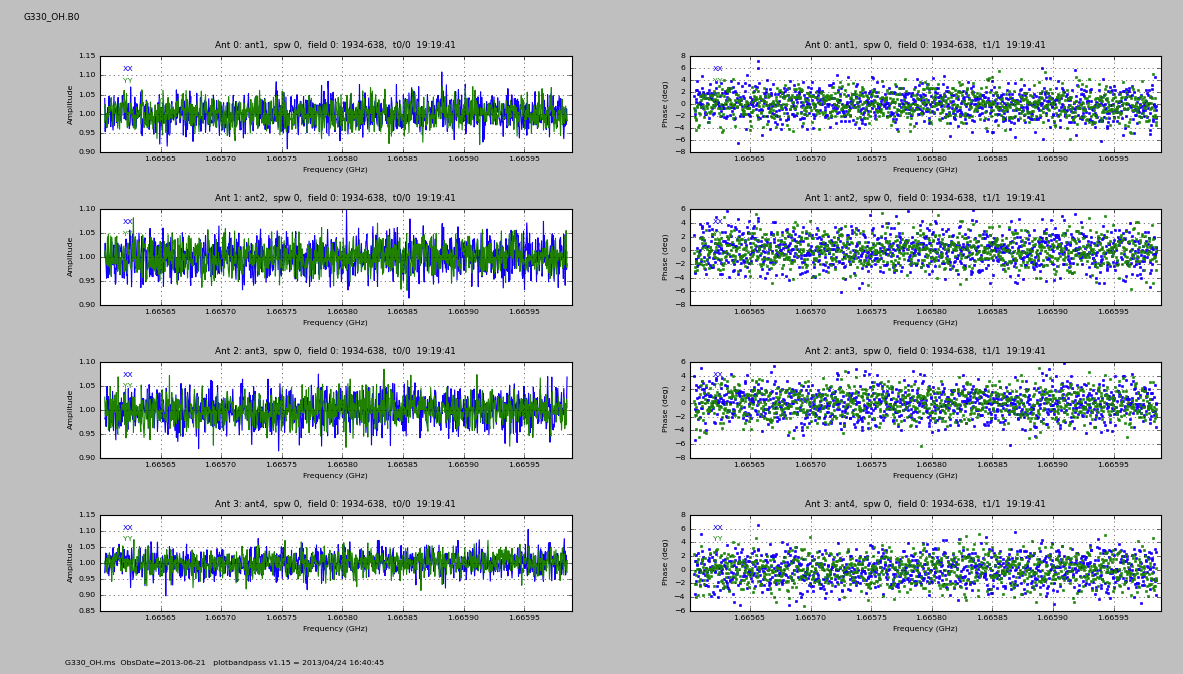
\includegraphics[width=\textwidth]{images/plotbandpass_b}
  \caption[]{The output of plotbandpass for a few antennas.}
  \forceversofloat
  \label{fig:plotbandpass_b}
\end{figure}

The problem with such narrow band observations is that we have increased noise.  Note that the
peak-to-peak amplitude variation is about 10\% and the phase variation is about 8 degrees.  However,
there is not much variation in the bandpass, so we can use a polynomial-based bandpass calibration.
Note below that we change bandtype to {\tt 'BPOLY'}. We can specify different orders of polynomial fit
for the phase and amplitude if necessary (Figure~\ref{fig:plotbandpass_bpoly}).

\begin{casacmd}
\begin{verbatim}
btable1 = prefix +'.B1'
bandpass(vis=msfile,
         caltable = btable1,
         field = b_cal,
         refant =ref_ant,
         solnorm = True,
         combine='scan',
         solint = 'inf',
         bandtype = 'BPOLY',
         degamp = 10,
         degphase = 10,
         minsnr = 5,
         gaintable = [gtable0],
         interp = ['nearest'])
\end{verbatim}
\end{casacmd}

\begin{figure}
  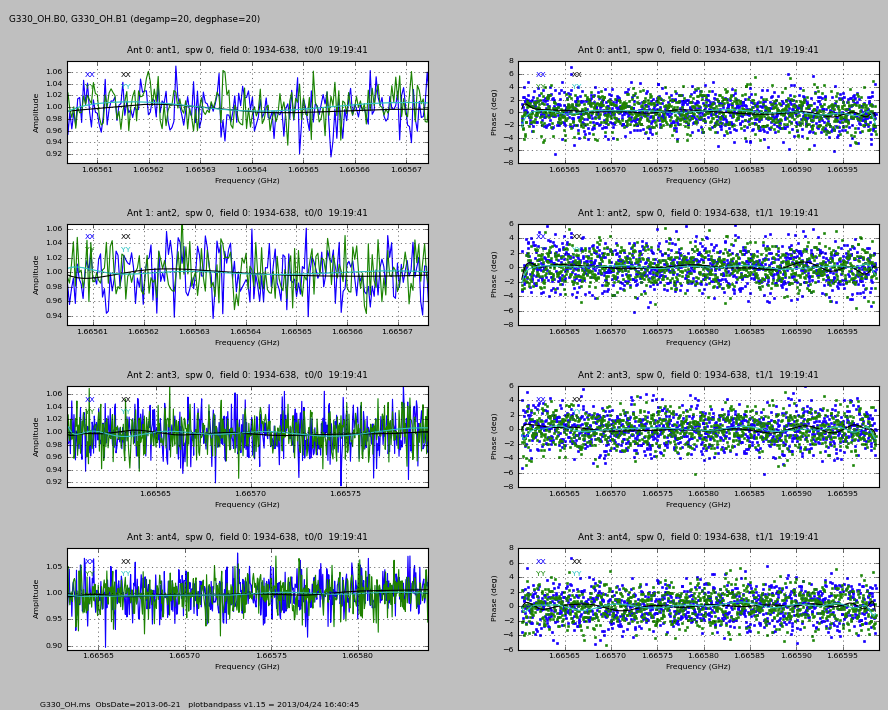
\includegraphics[width=\textwidth]{images/plotbandpass_bpoly}
  \caption[]{The output of plotbandpass with B and BPOLY solutions overlaid.}
  \forceversofloat
  \label{fig:plotbandpass_bpoly}
\end{figure}

Why is the bandpass calibration so important?  In spectral line observations we are interested in
source structure as a function of frequency, so we want to remove any spurious variations due to the
instrumental response. We may also want to subtract off continuum emission in order to simplify our
imaging and in this case we don't want there to be any residual continuum emission. How do we know if
we have sufficient signal to noise in our bandpass calibrator?  We typically want the rms noise from
the calibrator to be much less than the noise in the source.  We use calibrators with reasonably high
flux density, but spend less time on them than we do on our target sources, so its good to review
whether your observations satisfy the criterion that $I_{cal} \sqrt{t_{cal}}$ should be significantly
greater than $I_{target}\sqrt{t_{target}}$. In the case of this observation, the target actually has
quite a high continuum flux, and it will not be possible to meet this requirement without spending an
impractical amount of time on the bandpass calibrator.

Now we calibrate the gain on our flux calibrator, which in this observation happens to also be our
bandpass calibrator.

\begin{casacmd}
\begin{verbatim}
gaincal(vis = msfile,
        caltable = gtable1,
        field = f_cal,
        solint = 'inf',
        refant = ref_ant,
        gaintype = 'G',
        calmode = 'ap',
        solnorm = False,
        minsnr = 5,
        gaintable = [btable1],
        interp = ['nearest'])
\end{verbatim}
\end{casacmd}

Now check that there are no bad outliers in the gain calibration.

\begin{casacmd}
\begin{verbatim}
plotcal(caltable = gtable1,
            field = f_cal,
            xaxis = 'time',
            yaxis = 'amp',
            markersize=3,
            plotsymbol='.',
            iteration='antenna',
            subplot=421,
            fontsize=8)

plotcal(caltable = gtable1,
            field = f_cal,
            xaxis = 'time',
            yaxis = 'phase',
            markersize=3,
            plotsymbol='.',
            iteration='antenna',
            subplot=421,
            fontsize=8)
\end{verbatim}
\end{casacmd}

Calibrate the gains on the phase calibrator. Note that we append the solutions to the table containing
the gains on the flux calibrator.

\begin{casacmd}
\begin{verbatim}
gaincal(vis = msfile,
        caltable = gtable1,
        field = g_cal,
        solint = 'inf',
        refant = ref_ant,
        gaintype = 'G',
        calmode = 'ap',
        append = True,
        solnorm = False,
        minsnr = 5,
        gaintable = [btable1],
        interp = ['nearest'])
\end{verbatim}
\end{casacmd}

As usual, check the gain solutions and make sure that there's nothing nasty going on.  Next, we
transfer the flux scale from our flux calibrator to the gain calibrator. This will automatically
transfer the flux calibration to the target when we apply the calibrations.

\begin{casacmd}
\begin{verbatim}
fluxscale(vis=msfile,
          caltable = gtable1,
          fluxtable = ftable1,
          reference = f_cal,
          transfer = g_cal)
\end{verbatim}
\end{casacmd}

% \bigskip

\begin{casaoutput}
\begin{verbatim}
##########################################
##### Begin Task: fluxscale          #####
fluxscale(vis="G330_OH.ms",caltable="G330_OH.G1",
                fluxtable="G330_OH.fluxscale1",reference="1934-638",
                transfer="1613-586",listfile="",append=False,refspwmap=[-1],
                incremental=False, fitorder=1)
Opening MS: G330_OH.ms for calibration.
Initializing nominal selection to the whole MS.
Beginning fluxscale--(MSSelection version)-------
 Found reference field(s): 1934-638
 Found transfer field(s):  1613-586
 Flux density for 1613-586 in SpW=0 is: 1.01027 +/- 0.00741467 (SNR = 136.252, N = 14)
Storing result in G330_OH.fluxscale1
Writing solutions to table: G330_OH.fluxscale1
##### End Task: fluxscale            #####
##########################################
\end{verbatim}
\end{casaoutput}

Check that the derived flux is close to what is expected.  Now we are ready to apply the calibration
and get ready for imaging.

\begin{casacmd}
\begin{verbatim}
target = 'G330.89-0.36'
applycal(vis=msfile,
         field = target,
         gaintable = [btable1, ftable1],
         gainfield = [b_cal, g_cal],
         interp = ['nearest', 'linear'])
\end{verbatim}
\end{casacmd}

\begin{casacmd}
\begin{verbatim}
split_outputvis = target+'.split.ms'
split(vis = msfile,
      outputvis = split_outputvis,
      field = target,
      datacolumn = 'corrected')
\end{verbatim}
\end{casacmd}


\section{Velocity rest frames}

There are a few things that you need to do before you can dive in and start cleaning your image.
Since spectral line observations give us a lot of information about velocities of the objects that we
are observing, it is important to be clear on what reference frames we are using.  The apparent
frequency of a source, also known as the 'sky frequency', is influenced by Earth's rotation and
revolution around the Sun, the motion of our Solar System around the Galaxy, the movement of our
Galaxy within the Local Group and there is also motion against the cosmic microwave background.  The
various rest frames are listed in Table~\ref{tab:rest_frames}. At L-band, the sky frequency change by
up to 0.15 MHz during the course of a year.

The KAT-7 system does not do any Doppler corrections, so its rest frame is \textbf{topocentric}.  The
actual sky frequency of your source will vary from day to day and if you are observing with high
frequency resolution, you may even see your spectral line shifting during the course of a single day's
observation.  This is definitely the case for these hydroxyl maser observations.  We have a velocity
resolution of 68 m/s so we do see the source Doppler-shifted by Earth's rotation.

You will usually want to have your final data cubes output into a different rest frame. The velocity
frame to use depends on your science.  In the case of this dataset, we are looking at a Galactic star
formation region.  It is meaningfull in this case to work in the \textbf{Local Standard of Rest (LSR)
frame}.  There are actually two definitions of LSR, the kinematic LSR (LSRK) and dynamic LSR (LSRD).
Most of the time LSRK is used and is generally synomynous with LSR.  The other commonly used rest
frame is \textbf{barycentric}, and has mostly replaced the old heliocentric standard.

There are two ways to change rest frames in CASA.  The CLEAN task can change the reference frame of
the spectral axis which is fine if you don't have to worry about doppler shifts during the course of
the observation.  CVEL is a more general spectral regridding tool, which enables you to correct for
Doppler shifts, or change the channelisation on your data prior to imaging.  Doing the spectral
regridding before running CLEAN can save you time if you think you are going to be trying different
imaging settings.

\begin{table}
\caption{Velocity rest frames}
\label{tab:rest_frames}
\small
\begin{minipage}{1.2\textwidth}
\begin{tabular}{|l|l|l|l|}
\hline \rule[-2ex]{0pt}{5.5ex} Rest Frame Name & Rest frame & Corrects for & Max  \\
 &  &  & (km/s) \\ 
\hline \rule[-2ex]{0pt}{5.5ex} Topocentric & Telescope & Nothing &0 \\ 
\hline \rule[-2ex]{0pt}{5.5ex} Geocentric & Earth Centre & Earth Rotation & 0.5 \\
\hline \rule[-2ex]{0pt}{5.5ex} Earth-Moon & Earth-Moon    & Motion about &  0.013\\
Barycentric & centre of mass & Earth + Moon &\\
                   & & centre of mass & \\
\hline \rule[-2ex]{0pt}{5.5ex} Heliocentric & Centre of Sun & Earth orbital motion & 30 \\
\hline \rule[-2ex]{0pt}{5.5ex} Barycentric & Earth+Sun & Earth+Sun & 0.012 \\
 & centre of mass  & centre of mass & \\
\hline \rule[-2ex]{0pt}{5.5ex} Local standard of rest& Centre of mass& Solar motion rel & 20 \\
(LSR) & of local stars&to nearby stars &\\
\hline \rule[-2ex]{0pt}{5.5ex} Galactocentric & Centre of  & Milky Way & 230  \\
 &Milky Way & rotation &\\
\hline \rule[-2ex]{0pt}{5.5ex}Local Group  & Local Group  &  Milky Way& 100  \\
Barycentric &  centre of mass & motion & \\
\hline \rule[-2ex]{0pt}{5.5ex}  Virgocentric& Centre of the &Local Group  & 300 \\
 & Local Virgo & motion & \\
 & Supercluster & & \\
\hline \rule[-2ex]{0pt}{5.5ex} Cosmic Microwave & CMB & Local Supercluster & 600 \\
Background &   & motion & \\
\hline 
\end{tabular} 
\end{minipage}
\end{table}

\bigskip

\info{You can use the viewer to look at visibilities. Lets try it now.}

Figure~\ref{fig:doppler} shows a pretty severe shift over the course of the observations.  If we had
to image this dataset without correcting for the Doppler shift, we would end up blending our spectral
features together. We are going to be using CVEL to correct for the doppler shift, and at the same
time, change the velocity reference frame to the Local Standard of Rest ($V_{LSR}$).  Before we do
that, we need to set the line rest frequency in the measurement set.  The KAT-7 observation framework
does not make provision for setting the rest frequency in the data files so we shall have to do it
manually.  The rest frequency for this transition of OH is 1665.40184 MHz. We are going to open the
spectral window table and insert the rest frequency.  The default rest frequency in the file is
usually the central observing frequency.  Remember to close the file before continuing because it will
be locked until you do.

\begin{figure}
  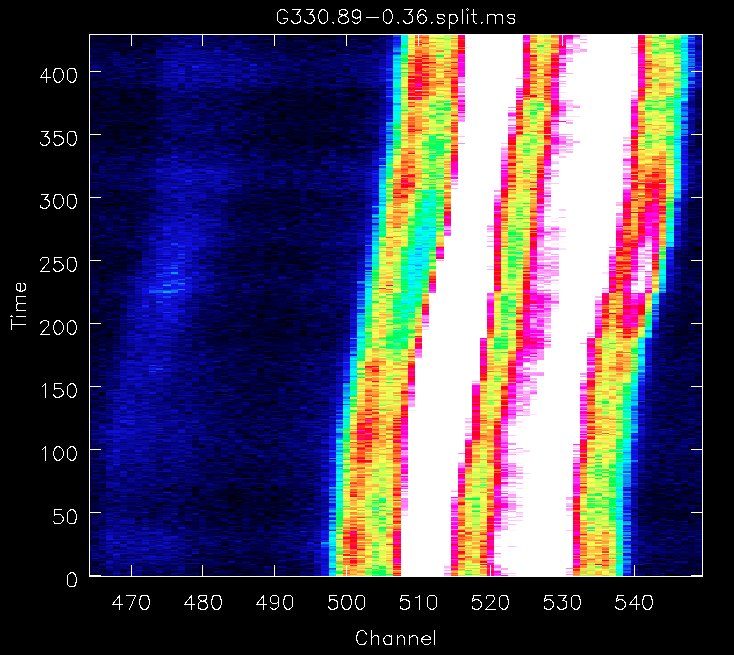
\includegraphics[width=\textwidth]{images/doppler_shift}
  \caption[]{A raster plot of visibilities on a single baseline. Note
how the spectral line is shifting through the channels over time.}
  \forceversofloat
  \label{fig:doppler}
\end{figure}

\begin{casacmd}
\begin{verbatim}
restfreq=1665.40184e6
tb.open(split_outputvis+'/SPECTRAL_WINDOW',
        nomodify=False)
tb.putcell('REF_FREQUENCY', 0, restfreq)
tb.close()
\end{verbatim}
\end{casacmd}

If run {\tt listobs} now you should see that the reference frequency has changed.  Next we run {\tt
cvel}.

\begin{casacmd}
\begin{verbatim}
freq_string =  str(restfreq/1e6)+'MHz'
cvel_outputvis = target+'.cvel.ms'
cvel(vis = split_outputvis,
     outputvis = cvel_outputvis,
     mode = 'velocity',
     interpolation = 'linear',
     outframe = 'LSRK',
     restfreq = freq_string)
\end{verbatim}
\end{casacmd}

\begin{figure}
  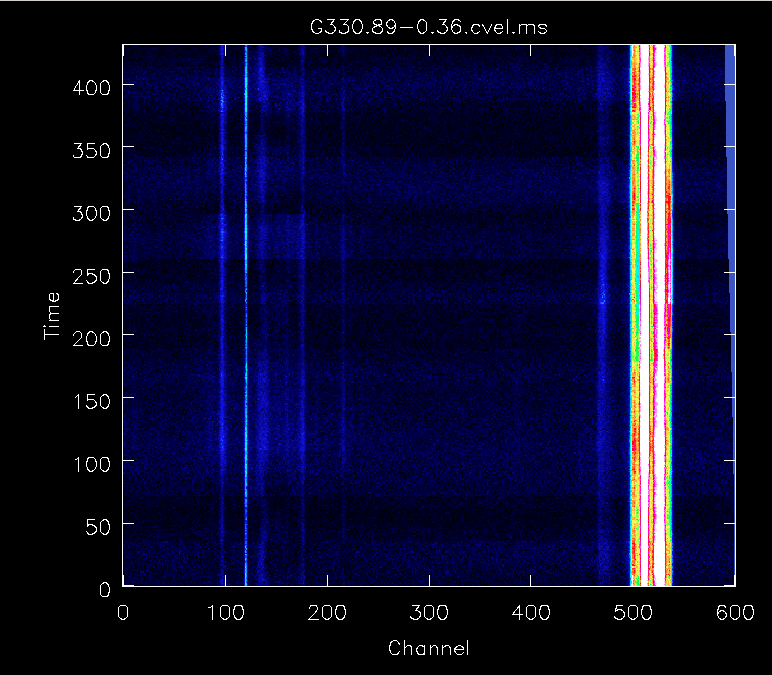
\includegraphics[width=\textwidth]{images/doppler_corrected}
  \caption[]{A raster plot of visibilities on a single baseline after doppler correction.}
  \forceversofloat
  \label{fig:doppler_corrected}
\end{figure}

This can take some time for a large dataset.  If you find yourself running low on disk space, you can
now delete the split file since we will use the cvel file from now on. Have a look at the spectral
lines using the viewer and convince yourself that we have removed the doppler shift. In
Figure~\ref{fig:doppler_corrected} you will see that the spectral lines now stay in the same channel.
Note that some of the edge channels are now missing data.  Make sure that you have split off
sufficient channels to account for this before you apply cvel.  We will lose about 10 channels in this
process. When you clean your datacube, you should make sure that these channels are not included. I
generally avoid this problem by setting the start velocity and number of channels for the output from
cvel such that I cover only the channels that I want to image.  This trick works well if you have
observations spread over more than a month, because the channel in which a particular velocity will be
present will vary over the year.  This brings your data into a common reference frame with consistent
channel numbers. If you don't know what these parameters should be, you can run cvel on the full
channel range, then examine the resulting file and rerun cvel with a smaller output range once you
know which velocity range is of interest.  Remember to leave sufficient line-free channels on either
side of your dataset for continuum subtraction.


\section{Continuum subtraction}

This particular field is of a massive star formation region.  The one degree field of view includes
several evolved HII regions as well as younger regions containing masers.  It will simplify the
cleaning process considerably if we can subtract the continuum and image it separately from the line
emission.  Lets have a look at a spectrum and see if we can establish the continuum baseline.  In the
case of these masers, the emission is so strong that we can see it in individual integrations, however
you need to be careful because there are also weaker features less than one Jy.  In the case of weaker
sources, we would need to average together all of the data in order to spot the emission. This works
well only if the source is close to the phase centre and not too extended.  The best way is to make a
dirty cube and examine this through the viewer in order to determine line channels. In the case of
extremely weak line sources you may even need to do some cleaning first before you can identify the
lines.

Lets have a quick look at the averaged spectrum.

\begin{casacmd}
\begin{verbatim}
plotms(vis=cvel_outputvis, 
       ydatacolumn = 'data',
       xaxis = 'channel',
       yaxis = 'amp',
       avgtime='1e8',
       avgscan=True)
\end{verbatim}
\end{casacmd}

There may be some emission around the last channels. It also turns out that this plot does not show
sufficient detail to figure out where the line emission is.  It will be much better to make a dirty
cube first and inspect the result to determine where we can place the continuum windows. To make a
dirty cube, we simple set the number of iterations of CLEAN to zero.

\begin{casacmd}
\begin{verbatim}
clean(vis = cvel_outputvis,
      imagename = 'dirty',
      mode = 'channel',
      outframe = 'LSRK',
      restfreq = freq_string,
      imsize = 256,
      cell='30arcsec',
      stokes = 'I',
      niter = 0,
      psfmode = 'hogbom',
      interactive = False,
      weighting = 'briggs')

viewer('dirty.image')
\end{verbatim}
\end{casacmd}

We have a reduced channel range in this dataset in order to keep the file sizes down, and as a result
most of the channels contain line emission.  Continuum subtraction is a lot easier in the original
4096 channel dataset.  Careful examination of the cube will show that the only line-free channels are
around 280 to 340. The continuum subtraction task will issue a warning about extrapolating over the
outer frequency ranges but will still do it.

\begin{casacmd}
\begin{verbatim}
cont_window = '0:280~340'
uvcontsub(vis=cvel_outputvis,
          fitspw = cont_window,
          fitorder = 1,
          want_cont = True)
\end{verbatim}
\end{casacmd}

Now you have two new measurement sets, one containing the continuum data, which you can image as
usual, and one containing the spectral data.  We do not expect to see any absorption features in this
field, so if you do see negative features, it may mean that the continuum subtraction has failed. You
can check this before going on to the laborious task of deconvolution by making a dirty cube of the
continuum-subtracted data.


\section{Finally, on to imaging}

Now we can start cleaning the spectral line cube.  Masers typically have angular sizes of the order of
milli-arcseconds and therefore  are not resolved with KAT-7.  However, there are five individual
sources of maser emission in this field of view.  Lets start the cleaning process.  You will notice
that we still specify the rest frequency even though we have already set it in the measurement set.
This is because of some inconsistencies in the way CASA handles spectral velocities - for now it is
safer to always specify the rest frequencies and the required output frame.

\begin{casacmd}
\begin{verbatim}
restfreq=1665.40184e6
freq_string =  str(restfreq/1e6)+'MHz'
contsub_vis = target+'.cvel.ms.contsub'
cube_namebase = target+'.cube.clean'

clean(vis = contsub_vis,
      imagename = cube_namebase,
      spw = '0:1~590',
      mode = 'channel',
      outframe = 'LSRK',
      restfreq = freq_string,
      imsize = 256,
      cell='30arcsec',
      stokes = 'I',
      threshold = '0.15Jy',
      niter = 20000,
      psfmode = 'hogbom',
      interactive = True,
      weighting = 'briggs')
\end{verbatim}
\end{casacmd}

If you find you are running out of time, try setting interactive to False and let CASA find its own
way.

Optional: Try cleaning the continuum.  Below are the commands to start the continuum cleaning.  Note
that I have dropped the last 11 channels to get rid of the empty channels that we were left with after
{\tt CVEL}.

\begin{casacmd}
\begin{verbatim}
cont_vis = target+'.cvel.ms.cont'
cont_image = target+'.cont.clean'

clean(vis=cont_vis,
      imagename = cont_image,
      spw = '0:0~590',
      imsize = 512,
      cell='30arcsec',
      stokes = 'I',
      threshold = '10mJy',
      niter = 5000,
      psfmode = 'hogbom',
      interactive = True,
      weighting = 'briggs')
\end{verbatim}
\end{casacmd}

You will notice that this field has a pretty complex structure, consisting of point sources as well as
more nebulous evolved HII regions. It is far better to clean this image using multi-scale clean, which
will fit for several size-scales. To set up multi-scale, we need to specify the scales, in number of
pixels, where 0 indicates a point source, 5 pixels is about one beam, and then we do a few multiples
of the beam, going up to 4 times the beam in this case.   Note that CASA will complain if the scales
are too large and then drop them.   If doing the cleaning non-interactively, it is good to also tell
CASA to stop when it starts creating too many negative components, otherwise things can go wrong very
quickly.

\caution{Warning: multiscale clean is a lot slower than the conventional clean because it repeats the
clean cycle for every scale specified and needs to re-scale the psf for every scale.  When setting
this task to non-interactive mode, and trying to clean down to 5 times the expected rms noise, this
takes almost 3 hours on a high-end desktop machine. This is also why we try to subtract the continuum
off in the uv-plane, since it speeds up imaging the OH masers considerably.
}

\begin{casacmd}
\begin{verbatim}
cont_image = target+'.cont.multiscale.clean'
clean(vis=cont_vis,
      imagename = cont_image,
      multiscale = [0, 5, 10, 15, 20],
      negcomponent = 1,
      spw = '0:0~590',
      imsize = 512,
      cell='30arcsec',
      stokes = 'I',
      threshold = '10mJy',
      niter = 5000,
      psfmode = 'hogbom',
      interactive = True,
      weighting = 'briggs')
\end{verbatim}
\end{casacmd}


\chapter{Troubleshooting and Support}
\label{ch:troubleshooting}

\section{Getting help}
\label{sec:getting-help}

In casapy, you can type {\tt help [commandname]} to get help in a particular command.

If you've encountered a problem, have a question, or would like to report a bug, please send an email
to our mailing list or visit our website.

\backmatter

% need this for bibtex
\newcommand{\aaps}{Astron. Astrophys. Suppl. Ser.}
\bibliographystyle{plainnat}
\bibliography{casa-bib}


\printindex

\end{document}
